\documentclass{beamer}

\mode<presentation> {
   \usetheme{Darmstadt}
  % \usetheme{Berlin}
  % \usetheme{Warsaw}
  % \usetheme{Singapore}
  % ou autre ...

  \setbeamercovered{transparent}
  % ou autre chose (il est également possible de supprimer cette ligne)
}

\usepackage[english]{babel}
% or autre comme par exemple \usepackage[english]{babel}
\usepackage{pstricks,pst-grad}
\usepackage{multicol}
\usepackage[utf8]{inputenc}
% or autre
\usepackage{exscale}
%\usepackage{authblk}
\usepackage{soul}
\usepackage[normalem]{ulem}
\usepackage{times}
\usepackage[T1]{fontenc}
\usepackage{natbib}
\usepackage{verbatim}
\usepackage{graphicx}
\usepackage{array, multirow}
\usepackage{color}
\usepackage{amsmath}
\usepackage{verbatim}
\usepackage{pgf}
\usepackage{tikz}
\usetikzlibrary{arrows,snakes,backgrounds,shapes}


\title[Titre court] % (facultatif, à utiliser uniquement si le titre de l'article est trop long)
{Ecology and Evolution of acute infectious diseases: the case of influenza}
%\subtitle {}

\author{Sébastien Ballesteros}

\institute[UMR 7625 Ecologie Evolution]
{
  UMR 7625 Ecologie Evolution\\
  Équipe Eco-Evolution mathématique\\
  ENS Ulm, UPMC
}

\date[Version courte] % (facultatif)
{18/12/2009 / Paris}

% À supprimer si vous ne voulez pas que la table des matières apparaisse
% au début de chaque sous-section :
% 
\AtBeginSubsection[] {
  \begin{frame}<beamer>{Contents}
  \begin{footnotesize}
    \tableofcontents[currentsection,currentsubsection]
  \end{footnotesize}
  \end{frame}
}

% Si vous souhaitez recouvrir vos transparents un à un,
% utilisez la commande suivante (pour plus d'info, voir la page 74 du manuel
% d'utilisation de Beamer (version 3.06) par Till Tantau) :

% \beamerdefaultoverlayspecification{<+->}


\begin{document}


\tikzstyle{naif} = [draw, fill=white, rectangle, minimum height=2em, minimum width=3em]
\tikzstyle{expo} = [draw, fill=blue!20, circle,minimum height=2em]
\tikzstyle{mut} = [draw, fill=red, circle,minimum height=2em]


\begin{frame}
  \titlepage
\end{frame}

\begin{frame}{Overview of the talk}

  \begin{footnotesize}
    \tableofcontents
  \end{footnotesize}

  % Vous pouvez, si vous le souhaiter ajouter l'option [pausesections]
\end{frame}


\section{Introduction~~~~~~~~~~~~~~~~~}

\subsection{General context: Phylodynamics}


\begin{frame}
  \frametitle{Phylodynamics: the melding of immunodynamics,
    epidemiology, and evolutionary biology}
  
  \begin{center}
%    \includegraphics<1>[width=0.9 \linewidth]{graph/phylodynamics_sout1.jpg}
%    \includegraphics<2>[width=0.9 \linewidth]{graph/phylodynamics_sout2.jpg}
%    \includegraphics<1>[width=0.9 \linewidth]{graph/phylodynamics_sout3.jpg}
%    \includegraphics<2>[width=0.9 \linewidth]{graph/phylodynamics_full.jpg}
    \includegraphics<1>[width=0.9 \linewidth]{graph/grenfell1.jpg}
    \includegraphics<2>[width=0.9 \linewidth]{graph/grenfell11.jpg}
    \includegraphics<3>[width=0.9 \linewidth]{graph/grenfell2.jpg}
    \includegraphics<4>[width=0.9 \linewidth]{graph/grenfell3.jpg}
    \includegraphics<5->[width=0.9 \linewidth]{graph/grenfell0.jpg}
  \end{center}

%  \includegraphics<1>[width=1 \linewidth]{graph/phylodynamics.jpg}    
%  \includegraphics<2>[width=1 \linewidth]{graph/phylodynamics_flu.jpg}    
%  \includegraphics<3>[width=1 \linewidth]{graph/phylodynamics_full.jpg}    

%  \begin{block}
%    \begin{footnotesize}
%       to explore how pathogen genetic variation is modulated
%      by host immunity, transmission bottlenecks and epidemic dynamics
%      to determine the wide range of pathogen phylogenies observed at
%      scales from individual host to population
%    \end{footnotesize}
%  \end{block}

\end{frame}


%\begin{frame}
%  \frametitle{A comparison of human infectious diseases dynamics}
%
%  \begin{center}
%    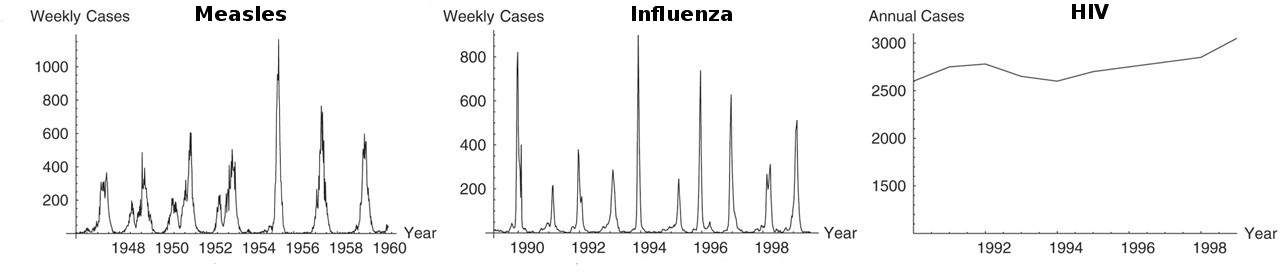
\includegraphics[width=1 \linewidth]{graph/grenfell_seb_cut.jpg}
%  \end{center}
%  \begin{flushright}
%    \begin{tiny} Adapted from Grenfell \textit{et al.} 2004 \end{tiny}
%  \end{flushright}
%
%\pause
%
%\begin{center}
%  \begin{tabular}{|c|c|c|c|}
%    \hline
%    & Measles & Influenza & HIV\\
%    \hline
%    duration of infection & $\sim15$ days & 1-7 days & years \\
%    \hline
%    vaccine update & none & ``every'' year & - \\
%    \hline	
%  \end{tabular}
%\end{center}
%
%\pause
%%tableau avec duree d'infection et mise a jour vaccinale
%\begin{block}{Question}
%  Evolutionary trajectories leading to major human infectious diseases
%\end{block}
%
%\end{frame}

\begin{frame}
  \frametitle{Evolutionary epidemiology 101}
  
  \begin{tikzpicture}[node distance=5cm, auto,>=latex', thick]<1>
    \tikzstyle{seb}=[->,draw=red, shorten >=1pt, >=stealth',semithick]
    \node [naif] (S) {$S$};
    \node [expo, right of=S] (I) {$I$};
    \node [expo, right of=I] (R) {$R$};
    \draw [->] (S) -- node {$\beta$: transmission rate} (I);
    \draw [->] (I) -- node{$\nu$: recovery rate}(R);
  \end{tikzpicture}

  \begin{columns}
    \begin{column}{0.6 \linewidth}
      \begin{footnotesize}
        \begin{align}
          \dot{S} &= \mu -\beta_1SI_1 -\beta_2SI_2 -\mu R \notag\\
          \dot{I_1} &= \beta_1SI_1 -\nu_1 I_1 -\mu I_1 \notag \\
          \dot{I_2} &= \beta_2SI_2 -\nu_2 I_2 -\mu I_2 \notag \\
          \dot{R} &= \nu_1 I_1 +\nu_2 I_2 -\mu R \notag
        \end{align}
      \end{footnotesize}      
    \end{column}
    \begin{column}{0.4 \linewidth}
      \begin{footnotesize}
        \begin{align*}
          S &\text{: Susceptible} \\
          I &\text{: Infected and infectious} \\
          R &\text{: Recovered and immunised} \\
          \mu &\text{: Birth and death rate} 
        \end{align*}
%        \begin{flushleft}
%          $S$: Susceptible\\
%          $I$: Infectious\\
%          $R$: Recovered\\
%          $\mu$: birth and death rate
%        \end{flushleft}
      \end{footnotesize} 
    \end{column}
  \end{columns}


  \pause
  \begin{block}{} %Basic reproductive number: $R_0$
    \begin{itemize}
    \item Under this model evolution maximises $R_0$
      \pause
    \item $R_0=\frac{\alert{\beta}}{\mu + \alert{\nu}}$ basic
      reproduction number: number of secondary infections produced by
      a single infectious host introduced in a fully susceptible
      population. \pause
    \item $\Rightarrow$ evolution toward \alert{chronic} ($\nu \to
      0$), highly transmissible diseases
    \end{itemize}
  \end{block}

\end{frame}

\begin{frame}
  \frametitle{Transmissibility and duration of infection are linked}
    % Evolutionary trade-off at two time scales between invasion and persistance

  \begin{columns}
    \begin{column}{0.6 \linewidth}<1->

      \begin{block}{Intra-host level}
        $\dot{P} = \alert{r}P - kXP$ \begin{footnotesize}(Pathogen load)\end{footnotesize}\\
        $\dot{X} = \alpha -dX +\gamma kXP$ \begin{footnotesize}(Immune response)\end{footnotesize}
      \end{block}
    \end{column}
    \begin{column}{0.4 \linewidth}<2->
      \includegraphics<2,3>[width=0.8 \linewidth]{graph/read.jpg}
      \includegraphics<4,5>[width=0.75 \linewidth]{graph/read2.jpg}
      %\includegraphics<5>[width=0.75 \linewidth]{acute_vs_chronic/acute0.pdf}
      \includegraphics<6->[width=0.85 \linewidth]{acute_vs_chronic/acute1.pdf}
    \end{column}
  \end{columns}

  \begin{alertblock}<3->{Population level}
%    Transmission potential ($\propto{R_0}$) proportionate to total
%    viral load%: $\beta=qP(t)$
    $R_0$ proportionate to total viral load%: $\beta=qP(t)$
  \end{alertblock}

  \begin{itemize}
  \item<5-> Maximise $R_0$ at the population level $\Rightarrow$
    maximise $r$ at the intra-host level $\Rightarrow$ short duration
    of infection $\Rightarrow$ violent epidemics and high risks of
    extinctions
  \item<7-> Pathogens evolve at the edge of their own
    extinction. Duration of infection is ultimately controled by
    population size
  \end{itemize}
  
\end{frame}

\begin{frame}
  \frametitle{Inclusion of antigenic variation at the intra-host level}
  
  Immune escape (\alert{antigenic variability}) at the intra-host level influences infection duration.\\
  
  \pause
  \begin{block}{Lange \& Ferguson 2009 model}
    \begin{itemize}
    \item Take into account antigenic variability and
      \alert{cross-immunity between pathogen strains} at the
      intra-host level.
    \item Shows how different classes of pathogens (measles, influenza
      and HIV-like) arise evolutionarily as fitness optima for
      different contact network structures and mode of transmission
      (constraint).
    \end{itemize}
  \end{block}

  \pause
  \begin{alertblock}{Question}
    How does antigenic diversity organise at the population level ?
  \end{alertblock}

\end{frame}

\begin{frame}
  \frametitle{How does antigenic diversity organise at the population level ?}
  
  \begin{center}
    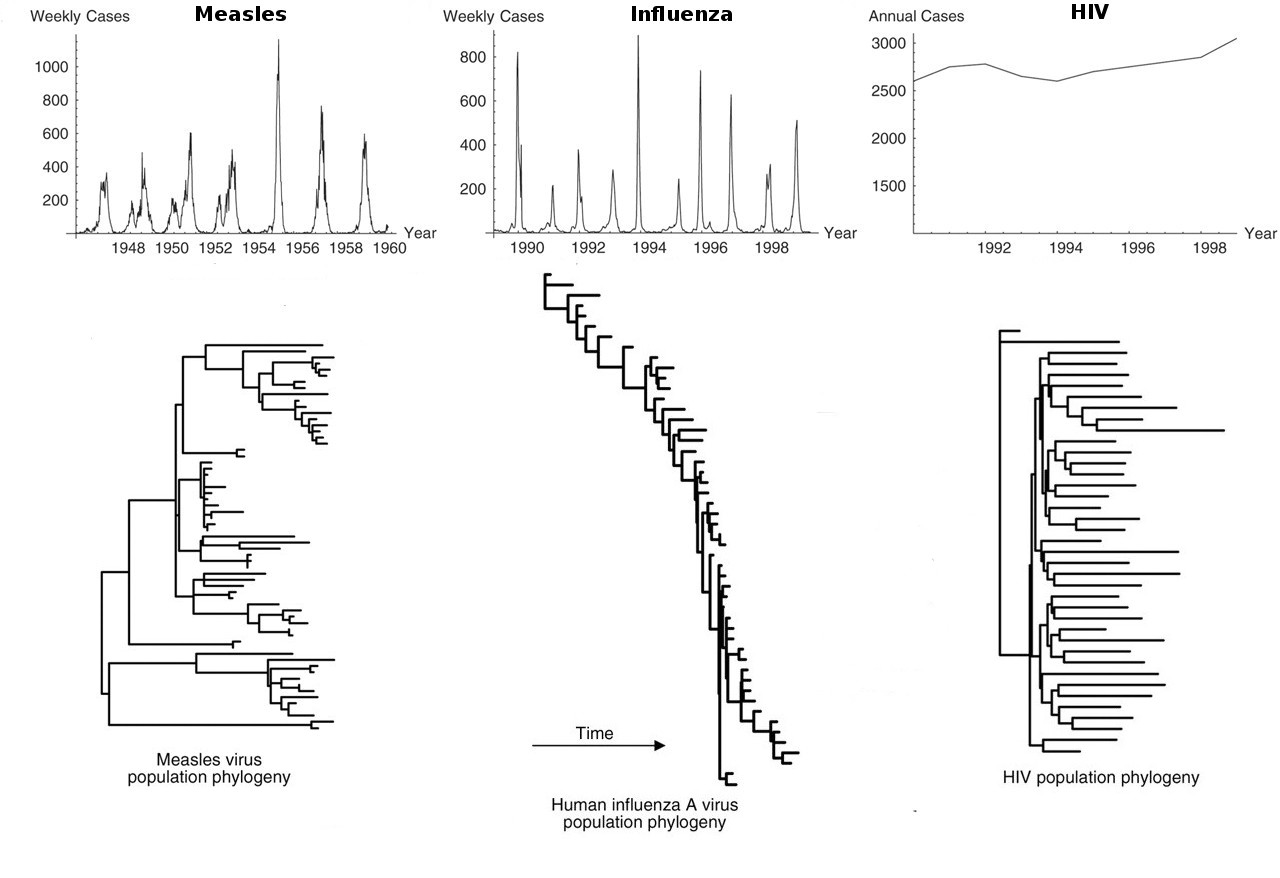
\includegraphics[width=0.9 \linewidth]{graph/phylodynamics_full2.jpg}
  \end{center}

\end{frame}


\subsection{Influenza as a case study}


\begin{frame}
  \frametitle{Structure and diversity of influenza A viruses}
  \begin{columns}[t]
    \begin{column}{0.3 \linewidth}
      \begin{center}
        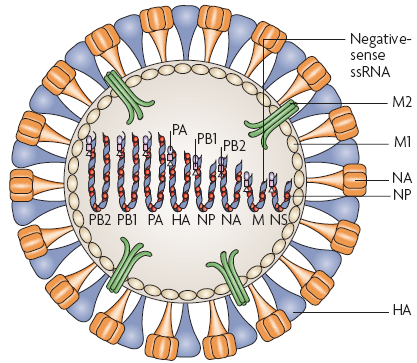
\includegraphics[width=1 \linewidth]{graph/struc.png}
      \end{center}
    \end{column}
    \begin{column}{0.7 \linewidth}
      %\pause
      \begin{itemize}
      \item ssRNA- viruses ; genome (13kb) composed of 8 segments (reassortment possible): \alert{strains}
        %\pause
      \item 2 main antigens: haemagglutinin (HA) and neuramidase (NA):
        \alert{subtypes HxNy}
        %\pause
      \item 3 phylogenetically and antigenically distinct viral \alert{types} A, B and C
      \end{itemize}
    \end{column}
  \end{columns}
%\vspace{0.1cm}
  %\pause
%Types and subtypes are introduced from (avian) reservoir during antigenic shifts.
%\pause
%\begin{block}{} We will focus on antigenic drift: change of strains within a given type or subtype.  \end{block}
\end{frame}

\begin{frame}
  \frametitle{Recent history of influenza pandemics}

  \begin{columns}
    \begin{column}{0.4 \linewidth}
      \begin{itemize}
      \item 16 HA and 9 NA in natural reservoir (aquatic birds)
      \item At least 103 of the 144 HA/NA combinations have been found 
      \end{itemize}
    \end{column}
    \begin{column}{0.7 \linewidth}
      \begin{center}
        \includegraphics<1>[width=0.6 \linewidth]{graph/hiromoto0.png}     
        \includegraphics<2>[width=0.6 \linewidth]{graph/hiromoto1.png}     
        \includegraphics<3>[width=0.6 \linewidth]{graph/hiromoto2.png}     
        \includegraphics<4>[width=0.6 \linewidth]{graph/hiromoto3.png}     
        \includegraphics<5->[width=0.6 \linewidth]{graph/hiromoto.png}     
      \end{center}
      
      \begin{tiny} Horimoto \& Kawaoka (2005) \end{tiny}
    \end{column}
  \end{columns}


\end{frame}


\begin{frame}
  \frametitle{Mexican Flu}

  \begin{center}
    \includegraphics<1>[width=0.7 \linewidth]{graph/news.png}    
    \includegraphics<2>[width=0.5 \linewidth]{graph/swine.png}    
    \only<2>{\begin{tiny} Neumann \textit{et al.} (2009) \end{tiny}}
  \end{center}

%  \begin{small}
%    \begin{itemize}
%    \item<2-> In the late 1990's reassortment between human H3N2,
%      north american avian and classical swine virus (H1N1) resulted
%      in a triple reaassortment H3N2 and H1N1 swine virus that have
%      since circulated in north american pig populations.
%    \item<3-> A triple reassortant swine virus reassorted with eurasian
%      avian-like swine virus (H1N1) resulting in the swine-origin
%      H1N1 influenza viruses that are now circulating in humans.
%    \end{itemize}
%  \end{small}

\end{frame}


%\begin{frame}
%  \frametitle{Causes of influenza recurrence}
%  \begin{columns}
%    \begin{column}{0.5 \linewidth}<1->
%      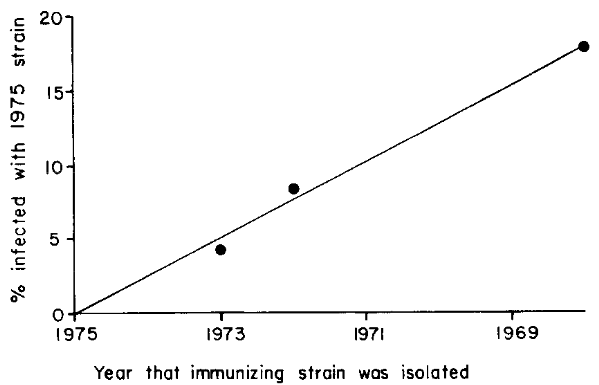
\includegraphics[width=0.8 \linewidth]{graph/pease2.png}\\
%      \begin{tiny} Gill and Murphy (1977) \end{tiny}
%    \end{column}
%    \begin{column}{0.5 \linewidth}<2->
%      Questions, result due to:
%        \begin{itemize}
%        \item antigenic evolution (immune escape) ?
%        \item loss of immunity ?
%        \end{itemize}
%    \end{column}
%  \end{columns}
%%  \pause
%  \begin{columns}
%    \begin{column}{0.5 \linewidth}<3->
%      \includegraphics<3->[width=0.8 \linewidth]{graph/pease1.png}\\
%      \begin{tiny} Potter \textit{et. al.} (1977) \end{tiny}
%    \end{column}
%    \begin{column}{0.5 \linewidth}<4->
%      \begin{block}{Conclusion}
%        immune escape is the main determinant of influenza A susceptible renewal
%      \end{block}
%    \end{column}
%  \end{columns}
%\end{frame}

\begin{frame}
  \frametitle{Ideal model for phylodynamics}

  \begin{center}
    \includegraphics<1>[height=0.7 \textwidth]{graph/eem1.pdf}
    \includegraphics<2>[height=0.7 \textwidth]{graph/eem2.pdf}
    \includegraphics<3>[height=0.7 \textwidth]{graph/eem3.pdf}
  \end{center}

\end{frame}


%\begin{frame}
%  \frametitle{Future}
%
%  \begin{center}
%    \includegraphics<1>[width=0.8 \linewidth]{graph/data_flu.jpg}
%    \includegraphics<2>[width=0.8 \linewidth]{graph/data_flu_question.jpg}
%  \end{center}
%
%  \begin{footnotesize}
%    Data:~\url{http://websenti.b3e.jussieu.fr/sentiweb/}
%  \end{footnotesize}
%
%  \begin{itemize}
%  \item<1-> Until April 2009 type A \alert{H3N2} and H1N1 subtypes
%    were co-circulating with type B influenza.
%  \item<2-> Current data suggest replacement of these subtype by the
%    new animal-origin pandemic H1N1 subtype
%  \end{itemize}
%
%\end{frame}


\subsection{Explaining influenza phylodynamics}

%\begin{frame}
%  \frametitle{The cause of recurrence: antigenic drift}
%  \begin{columns}
%    \begin{column}{0.5 \linewidth}<1->
%      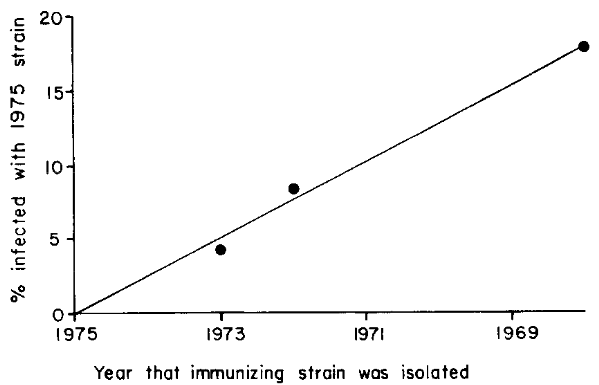
\includegraphics[width=0.8 \linewidth]{graph/pease2.png}\\
%      \begin{tiny} Gill and Murphy (1977) \end{tiny}
%    \end{column}
%    \begin{column}{0.5 \linewidth}<2->
%      Questions, result due to:
%        \begin{itemize}
%        \item antigenic evolution (immune escape) ?
%        \item loss of immunity ?
%        \end{itemize}
%    \end{column}
%  \end{columns}
%%  \pause
%  \begin{columns}
%    \begin{column}{0.5 \linewidth}<3->
%      \includegraphics<3->[width=0.8 \linewidth]{graph/pease1.png}\\
%      \begin{tiny} Potter \textit{et. al.} (1977) \end{tiny}
%    \end{column}
%    \begin{column}{0.5 \linewidth}<4->
%      \begin{block}{Conclusion}
%        immune escape is the main determinant of influenza A susceptible renewal
%      \end{block}
%    \end{column}
%  \end{columns}
%\end{frame}
%
%
%
%\begin{frame}
%  \frametitle{The genetic signature of antigenic drift}
%  \includegraphics<1->[height=0.5 \textwidth]{graph/fitch.png}
%  \begin{tiny} Fitch \textit{et. al.} (1997) \end{tiny}
%
%  %\begin{block}{} genetic drift is gradual \end{block}
%\end{frame}



\begin{frame}
  \frametitle{Reproducing influenza phylodynamics}

  %The Bitstring model (Girvan \textit{et al.} 2002)
  \includegraphics<1>[width=1 \linewidth]{graph/bitstring1.pdf}
  \includegraphics<2>[width=1 \linewidth]{graph/bitstring2.pdf}
  \includegraphics<3->[width=1 \linewidth]{graph/bitstring.pdf}

  \vspace*{0.5cm}

  \begin{columns}
    \begin{column}{0.35 \linewidth}
      \includegraphics<4->[height=1 \textwidth]{graph/ferg.png}

\only<4->{
      \begin{tiny}
        Ferguson \textit{et al.} (2003)
      \end{tiny}}
    \end{column}
    \begin{column}{0.65 \linewidth}
      \begin{block}<4->{Results}
        \alert{Explosive diversity of strains} and
        unrealistically high incidence
      \end{block}
      \begin{alertblock}<5->{Key theoretical question}
        How to restrict strains diversity ?
      \end{alertblock}
      
    \end{column}
  \end{columns}
  
\end{frame}

%\begin{frame}
%  \frametitle{Reproducing influenza phylodynamics}
%
%  \begin{itemize}
%  \item Basic \alert{multi-strains models} using high dimensional
%    antigenic space and gradual antigenic evolution reveal
%    \alert{explosive diversity of strains} and unrealistically high
%    disease incidence.
%  \end{itemize}
%  
%  \begin{columns}
%    \begin{column}{0.6 \linewidth}
%      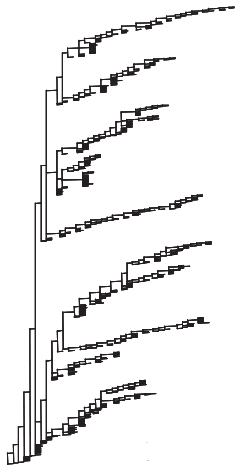
\includegraphics[height=0.7 \textwidth]{graph/ferg.png}      
%
%      \begin{tiny}
%        Ferguson \textit{et al.} (2003)
%      \end{tiny}   
%    \end{column}
%    \begin{column}{0.4 \linewidth}
%      \begin{alertblock}<2->{Key theoretical question}
%        How to restrict strains diversity ?
%      \end{alertblock}
%    \end{column}
% 
%  \end{columns}
%\end{frame}


\begin{frame}
  \frametitle{How to limit strains diversity ? \\1- Temporary strain-transcending immunity}
  To limit strains diversity models have had to invoke :
  \begin{enumerate}
  \item<1-> \alert{Temporary strain-transcending immunity} (density
    dependence) and a form of heterogeneity (Ferguson et al. 2003, Xia
    et al. 2005).
  \end{enumerate}

  \begin{columns}
    \begin{column}{0.7 \linewidth}
      \includegraphics<1,2,3->[height=0.5 \textwidth]{graph/ferg.png}
      \includegraphics<2->[height=0.5 \textwidth]{graph/fergQ3.pdf}
%      \includegraphics<3->[height=0.5 \textwidth]{graph/fergQ.png}

      \begin{tiny}
        Ferguson \textit{et al.} (2003)
      \end{tiny}
    \end{column}
    \begin{column}{0.3 \linewidth}
      \begin{block}<3->{Controversy}
        Few empirical support ?
      \end{block}
    \end{column}
  \end{columns}

\end{frame}


%\begin{frame}
%  \frametitle{How to limit strains diversity ? (2)}
%  To limit strains diversity models have had to invoke :
%  \begin{enumerate}
%  \item<1-> Temporary strain-transcending immunity (density
%    dependence) and a form of heterogeneity (Ferguson et al. 2003, Xia
%    et al. 2005).  Few empirical support ?
%%  \item<2-> That the virus continually reuses a limited number of
%%    antigenic combinations (Recker et. al. 2007)
%  \item<1-> That influenza A main antigen (hemagglutinin) evolves in a
%    punctuated manner, punctuated immune escape resulting in selective
%    sweeps (Koelle et al. 2006). \alert{Non linear genotype to
%      phenotype map}
%  \end{enumerate}
%\end{frame}

\begin{frame}
  \frametitle{How to limit strains diversity ? \\2- Linking genotype to phenotype}
  \begin{columns}
    \begin{column}{0.5 \linewidth}
      \begin{center}
        \includegraphics<1,2,3>[height=0.8 \textwidth]{graph/fitch.png}
        \includegraphics<4->[height=0.8 \textwidth]{graph/smith1.jpeg}
        \only<4->{\begin{tiny} Smith \textit{et. al.} (2004) \end{tiny}}
       \end{center}
    \end{column}
    \begin{column}{0.5 \linewidth}
      \begin{center}
        \includegraphics<2>[height=0.7 \textwidth]{graph/flu_hemagl.jpg}
        \includegraphics<3->[height=0.8 \textwidth]{graph/smith2.jpeg}
        \only<3->{\begin{tiny} Smith \textit{et. al.} (2004) \end{tiny}}
       \end{center}
    \end{column}
  \end{columns}

  \begin{block}<4->{Conclusion}
      Antigenic mapping reveals that the evolution of influenza A main antigen (haemagglutinin, HA) is punctuated with \alert{antigenic clusters} jumps.
  \end{block}
\end{frame}


\begin{frame}
  \frametitle{How to limit strains diversity ? \\2- Punctuated immune escape}
  
  \begin{center}
    %\includegraphics<1>[height=0.4 \linewidth]{graph/koelle.jpg}
    \includegraphics<1->[height=0.4 \linewidth]{graph/koelle_tr_ink.pdf}
  \end{center}
  \begin{tiny}
    Koelle et al. 2006
  \end{tiny}

  \begin{itemize}
  \item<1-> Antigenic cluster transitions induce selective sweeps
  \item<2-> \alert{Paradigm shifts} in influenza antigenic evolution 
  \end{itemize}
\end{frame}


\subsection{Objectives}

\begin{frame}
  \frametitle{Objectives}
  \begin{itemize}
  \item<1-> Current hypothesis explaining influenza phylodynamics are
    supported by complex simulations
  \item<2-> It renders difficult to disentangle various processes shaping
    the observed dynamics and the consequences of modelling assumptions
  \end{itemize}


  \begin{block}<3->{Our aims}
    \begin{itemize}
    \item<3-> to develop simple as possible models to determine a minimal
      theory for influenza
    \item<4-> keeping the framework sufficiently tractable to allow
      confrontation to epidemiological time-series and statistical
      inference
    \end{itemize}
  \end{block}

\end{frame}


\section[Multi-strains models]{Effect of classical multi-strains models on transient
  invasion dynamics}

\subsection{Multi-strains models}


\begin{frame}
  \frametitle{Different hypothesis to model partial cross-immunity}

  \begin{columns}
    \begin{column}{0.6 \linewidth}
      \begin{itemize}
      \item<1-> History Based models
        \begin{itemize}
        \item<1-> Reduced Susceptibility (HBRS)
        \item<1-> Reduced Infectivity (HBRI)
        \item<1-> Reduced Transmissibility (Gupta)
        \end{itemize}
      \item<1-> Status Based models
        \begin{itemize}
        \item<1-> Reduced Susceptibility (SBRS)
        \item<1-> Reduced Infectivity (SBRI)
        \end{itemize}
      \end{itemize}      
    \end{column}
    \begin{column}{0.4 \linewidth}
      \includegraphics<3->[width=0.8 \linewidth]{graph/tux2.pdf} 
    \end{column}
  \end{columns}

  \begin{block}<2->{Constraints}
    For a system of $K$ strains, the number of state variables scales
    with $\sum_k \binom{K}{k}=2^K$.\\
    \pause
    For a general antigenic space, only the \alert{SBRI model} is
    amenable to dimension reduction with 2K states variable for $K$
    strains. Influenza A punctuated evolution relies exclusively on
    this model.
  \end{block}

%  \begin{columns}
%    \begin{column}<1->{0.5 \linewidth}
%      \begin{center}
%        \textbf{History based model}
%      \end{center}
%      \vspace{0.1 cm}
%      \begin{tikzpicture}[node distance=1.4cm, inner sep=0pt, minimum size=8mm]
%    \tikzstyle{seb}=[rectangle, fill=red, draw=gray, text=black] \tikzstyle{I1}=[->, draw=red, shorten >=1pt, >=stealth',semithick]     \tikzstyle{I2}=[->,draw=blue, shorten >=1pt, >=stealth',semithick] \tikzstyle{g1}=[->,shorten >=1pt, >=stealth',semithick]     \tikzstyle{g2}=[->,shorten >=1pt, >=stealth',semithick]
%
%    \node[seb] (R0) {$R_\varnothing$};
%    \node[seb] (R1) [above of=R0] {$R_1$};
%    \node[seb] (R2) [below of=R0] {$R_2$};
%    \node[seb] (R12) [right of=R0] {$R_{12}$};
%
%    \draw[I1] (R0) to node[auto] {\begin{tiny}$\beta R_\varnothing I^1$\end{tiny}} (R1);
%    \draw[I2] (R0) to node[auto,swap]     {\begin{tiny}$\beta R_\varnothing I^2$\end{tiny}} (R2);
%    \draw[I2] (R1.east) to node[auto] {\begin{tiny}$\sigma \beta R_1 I^2$\end{tiny}} (R12.west);
%    \draw[I1] (R2.east) to node[auto,swap] {\begin{tiny}$\sigma \beta R_2 I^1$\end{tiny}}     (R12.west);
%  \end{tikzpicture}
%
%  % \begin{itemize}
%  % \item Reduced susceptibility
%  % \item Reduced infectivity (not shown)
%  % \end{itemize}
%  
%    \end{column}
%    \begin{column}<2->{0.5 \linewidth}
%      \begin{center}
%        \textbf{Status based model}
%      \end{center}
%      \vspace{0.1 cm}
%
%  \begin{tikzpicture}[node distance=1.4cm, inner sep=0pt, minimum size=8mm]
%    \tikzstyle{seb}=[rectangle, fill=red, draw=gray, text=black] \tikzstyle{I1}=[->, draw=red, shorten >=1pt, >=stealth',semithick]     \tikzstyle{I2}=[->,draw=blue, shorten >=1pt, >=stealth',semithick] \tikzstyle{g1}=[->,shorten >=1pt, >=stealth',semithick]     \tikzstyle{g2}=[->,shorten >=1pt, >=stealth',semithick]
%
%    \node[seb] (R0) {$R_\varnothing$};
%    \node[seb] (R1) [above of=R0] {$R_1$};
%    \node[seb] (R2) [below of=R0] {$R_2$};
%    \node[seb] (R12) [right of=R0] {$R_{12}$};
%
%    \draw[I1] (R0) to node[auto] {\begin{tiny}$(1-\sigma') \beta R_\varnothing I^1$\end{tiny}} (R1);
%    \draw[I2] (R0) to node[auto,swap]     {\begin{tiny}$(1-\sigma') \beta R_\varnothing I^2$\end{tiny}} (R2); 
%    \draw[I2] (R1.east) to node[auto] {\begin{tiny}$\beta R_1         I^2$\end{tiny}} ( R12.west);
%    \draw[I1] (R2.east) to node[auto,swap] {\begin{tiny}$\beta R_2 I^1$\end{tiny}}     ( R12.west);
%    \draw[I1] ([yshift=+1mm] R0.east) to node[auto] {\begin{tiny}$\sigma' \beta R_\varnothing I^1$\end{tiny}} ([yshift=+1mm] R12.west); 
%    \draw[I2]     ([yshift=-1mm] R0.east) to node[auto,swap] {\begin{tiny}$\sigma' \beta R_\varnothing I^2$\end{tiny}} ([yshift=-1mm] R12.west);
%  \end{tikzpicture}
%
%  % \begin{itemize}
%  % \item Reduced susceptibility
%  % \item Reduced infectivity (not shown)
%  % \end{itemize}
%    \end{column}
%
%  \end{columns}
%
\end{frame}


\begin{frame}
  \frametitle{The serial $SIR$ framework for influenza} 

  \begin{block}<1->{Aim}
    comparison of the consequences of status based, history based,
    reduced susceptibility and infectivity assumptions on the
    \alert{transient} dynamics of antigenic clusters replacement.
  \end{block}

  \begin{columns}
    \begin{column}{0.4 \linewidth}
      \includegraphics<1->[width=0.8 \textwidth]{graph/smith1.jpeg}      
    \end{column}
    \begin{column}{0.6 \linewidth}
      \begin{itemize}
      \item<2-> We take an adaptive dynamics framework
      \item<2-> We study the invasion of a mutant antigenic cluster
        within a population where a resident antigenic cluster is at the
        endemic equilibrium
      \end{itemize}
    \end{column}
  \end{columns}

\end{frame}


\begin{frame}
  \frametitle{Comparison of invasion dynamics}
  
  \begin{center}
    \includegraphics<1>[width=0.5 \linewidth]{traj_theoretical12/compare1.pdf}
    \includegraphics<2->[width=0.5 \linewidth]{traj_theoretical12/compare2.pdf}
  \end{center}

  \begin{block}<2->{}
    Antigenic clusters replacement apears to be possible only for the
    $SBRI$ model. \alert{Why ?}
  \end{block}

\end{frame}

%\begin{frame}
%  \frametitle{Invasion condition of the mutant cluster}
%
%  \begin{itemize}
%  \item<1-> For status based model, in both $SBRI$ and $SBRS$ models, the invasion condition can be deduced from:  
%$$\left. \frac{d I^2}{d t} \right|_{R_\varnothing^*, R_1^*} = (\beta_2 R_\varnothing^*  + \beta_2 R_1^* -\nu -\mu) I^2$$
%\item<1-> In the history based framework, the previous approach is not
%  feasible for the model $HBRI$. The basic reproduction ratio $R_0$ is
%  then calculated as the dominant egeinvalues of the linear next
%  generation operator and is identical for all the models.
%%In both $HBRS$ and $HBRI$ model the dominant eigenvalue is:
%%$$R_0^{inv} = \frac{\beta_2 SS^* + \beta_2 s x RS^* +\beta_2 s x IS^*}{\mu+\nu}$$
%  \end{itemize}
%\end{frame}


\begin{frame}
  \frametitle{Initial speed of invasion of the mutant cluster}
 
  \begin{center}
    \begin{tabular}{|l|l|}
      \hline
      model & $R_0^{inv}$ \\
      \hline
      $SBRI$ & $1 + \sigma(R_0 -1)/\alert{((1-\sigma) (R_0-1) +1)}$ \\
      \hline
      all others & $1 + \sigma(R_0 -1)$\\
      \hline
    \end{tabular}
  \end{center}

$\sigma \in [0,1]$: immune escape

%\pause

  \begin{block}{}
    The $SBRI$ model assumption appears to reduce the initial speed of
    invasion of the mutant cluster.  \alert{Why ?}
  \end{block}

  \pause
  \begin{alertblock}{To understand why}
    Re-derivation of the main multi-strains models within a unified
    framework based on immunity variables
  \end{alertblock}
\end{frame}





\begin{frame}
  \frametitle{Unifying framework with immunity  variables ($R_J$): History~based~models}

  \begin{itemize}
  \item Reduced susceptibility (HBRS)
  \end{itemize}
  \begin{tikzpicture}[node distance=2cm, inner sep=0pt, minimum size=8mm]
    \tikzstyle{seb0}=[rectangle, fill=white, draw=gray, text=black]
    \tikzstyle{seb}=[rectangle, fill=blue!20, draw=gray, text=black]
    \tikzstyle{seb2}=[rectangle, fill=red, draw=gray, text=black]
    \tikzstyle{I1}=[->, draw=blue, shorten >=1pt, >=stealth',semithick]  
    \tikzstyle{I2}=[->,draw=red, shorten >=1pt, >=stealth',semithick] 
    \tikzstyle{g1}=[->,shorten >=1pt, >=stealth',semithick]     \tikzstyle{g2}=[->,shorten >=1pt, >=stealth',semithick]
    
    \node[seb0] (R0) {$R_\varnothing$};
    \node[seb] (I1) [right of=R0] {$I^1$};
    \node[seb] (R1) [right of=I1] {$R_{1}$};
    \draw[I1] (R0) to node[auto] {\begin{tiny}$\beta R_\varnothing I^1$\end{tiny}} (I1);
    \draw[g1] (I1) to node[auto] {\begin{tiny}$\nu$\end{tiny}} (R1);
    
    \pause

    \node[seb2] (I2) [right of=R1] {$I^2_1$};
    \node[seb2] (R12) [right of=I2] {$R_{12}$};
    \draw[I2] (R1) to node[auto] {\begin{tiny}$\alert{\sigma} \beta R_1 (I^2_\varnothing +I^2_1)$\end{tiny}} (I2);
    \draw[g1] (I2) to node[auto] {\begin{tiny}$\nu$\end{tiny}} (R12);

  \end{tikzpicture}

  \pause
  \begin{itemize}
  \item Reduced infectiosity (HBRI)
    \begin{itemize}
    \item 2 kind of host infected by strain 2.
      %\pause
    \item $R_\varnothing \to I^2_\varnothing$ and $R_1 \to I^2_1$
      %\pause
    \item different contribution to the force of infection:
      $\beta_2(I^2_\varnothing + \alert{\sigma} I^2_1)$
    \end{itemize}
  \end{itemize}


  %\pause
  \begin{itemize}
  \item Reduced transmissibility (Gupta) 
  \end{itemize}

  \begin{tikzpicture}[node distance=2cm, inner sep=0pt, minimum size=8mm]
    \tikzstyle{seb0}=[rectangle, fill=white, draw=gray, text=black]
    \tikzstyle{seb}=[rectangle, fill=blue!20, draw=gray, text=black]
    \tikzstyle{seb2}=[rectangle, fill=red, draw=gray, text=black]
    \tikzstyle{I1}=[->, draw=blue, shorten >=1pt, >=stealth',semithick]  
    \tikzstyle{I2}=[->,draw=red, shorten >=1pt, >=stealth',semithick] 
    \tikzstyle{g1}=[->,shorten >=1pt, >=stealth',semithick]     \tikzstyle{g2}=[->,shorten >=1pt, >=stealth',semithick]

    \node[seb0] (R0) {$R_\varnothing$};
    \node[seb] (I1) [right of=R0] {$I^1$};
    \node[seb] (R1) [right of=I1] {$R_{1}$};
    \draw[I1] (R0) to node[auto] {\begin{tiny}$\beta R_\varnothing I^1$\end{tiny}} (I1);
    \draw[g1] (I1) to node[auto] {\begin{tiny}$\nu$\end{tiny}} (R1);

    %\pause

%    \node[seb2] (I20) [above of=I1] {$I^2_\varnothing$};
    \node[seb2] (I2) [right of=R1] {$I^2_1$};
    \node[seb2] (R12) [right of=I2] {$R_{12}$};
    \draw[I2] (R1) to node[auto] {\begin{tiny}$\alert{\sigma} \beta R_1 (I^2_\varnothing + I^2_1) $\end{tiny}} (I2);
%    \draw[g1] (R1) to node[auto] {\begin{tiny}$\alert{(1-\sigma)} \beta R_1 (I^2_\varnothing +I^2_1) $\end{tiny}} (R12);
    \draw[g1] (I2) to node[auto] {\begin{tiny}$\nu$\end{tiny}} (R12);
    \draw[g1](R1) -- +(0,-1) -| node[near start,above] {\begin{tiny}$\alert{(1-\sigma)} \beta R_1 (I^2_\varnothing +I^2_1) $\end{tiny}} (R12);
  \end{tikzpicture}

\end{frame}



\begin{frame}
  \frametitle{Unifying framework with immunity  variables ($R_J$): Status~based~models}

  \begin{columns}
    \begin{column}{0.5 \linewidth}<1->
      \begin{itemize}
      \item Reduced susceptibility (SBRS)
      \end{itemize}
      \vspace{0.1 cm}
      \begin{tikzpicture}[node distance=2cm, inner sep=0pt, minimum size=8mm]
        \tikzstyle{seb0}=[rectangle, fill=white, draw=gray, text=black]
        \tikzstyle{seb}=[rectangle, fill=blue!20, draw=gray, text=black]
        \tikzstyle{seb2}=[rectangle, fill=red, draw=gray, text=black]
        \tikzstyle{I1}=[->, draw=blue, shorten >=1pt, >=stealth',semithick]  
        \tikzstyle{I2}=[->,draw=red, shorten >=1pt, >=stealth',semithick] 
        \tikzstyle{g1}=[->,shorten >=1pt, >=stealth',semithick]     \tikzstyle{g2}=[->,shorten >=1pt, >=stealth',semithick]
        
        \node[seb0] (R0) {$R_\varnothing$};
        \node[seb] (R1) [right of=R0] {$R_{1}$};
        \node[seb2] (R12) [below of=R1] {$R_{12}$};
        \draw[I1] (R0) to node[auto] {\begin{tiny}$(1-\sigma') \beta R_\varnothing I^1$\end{tiny}} (R1);
        \draw[I1] (R0) to node[auto] {\begin{tiny}$\sigma' \beta R_\varnothing I^1$\end{tiny}} (R12);
      \end{tikzpicture}
    \end{column}

    \begin{column}{0.5 \linewidth}<2->
      
      \begin{itemize}
      \item Reduced Infectivity \\(SBRI)
      \end{itemize}
      \vspace{0.1 cm}
      \begin{tikzpicture}[node distance=2cm, inner sep=0pt, minimum size=8mm]
        \tikzstyle{seb0}=[rectangle, fill=white, draw=gray, text=black]
        \tikzstyle{seb}=[rectangle, fill=blue!20, draw=gray, text=black]
        \tikzstyle{seb2}=[rectangle, fill=red, draw=gray, text=black]
        \tikzstyle{I1}=[->, draw=blue, shorten >=1pt, >=stealth',semithick]  
        \tikzstyle{I2}=[->,draw=red, shorten >=1pt, >=stealth',semithick] 
        \tikzstyle{g1}=[->,shorten >=1pt, >=stealth',semithick]     \tikzstyle{g2}=[->,shorten >=1pt, >=stealth',semithick]
        
        \node[seb0] (R0) {$R_\varnothing$};
        \node[seb] (R1) [right of=R0] {$R_{1}$};
        \node[seb2] (R12) [below of=R1] {$R_{12}$};
        \draw[I1] (R0) to node[auto] {\begin{tiny}$(1-\sigma') \beta R_\varnothing I^1$\end{tiny}} (R1);
        \draw[I1] (R0) to node[auto] {\begin{tiny}$\sigma'
            \beta R_\varnothing I^1$\end{tiny}} (R12);
        \draw[I2] (R1) to node[auto] {\begin{tiny}$\alert{\sigma' \beta R_1 I^1}$\end{tiny}} (R12);
      \end{tikzpicture}
    \end{column}
  \end{columns}

%  \begin{block}{}
%    Status determined at the time of infection
%  \end{block}
\end{frame}



\begin{frame}
  \frametitle{Reinfection and cross-immune boosting is necessary for
    dimensionality reduction for the SBRI model}

  \begin{columns}
    \begin{column}{0.7 \linewidth}<1->
      \begin{tiny}
        \begin{align}
          \dot{R_\varnothing} & = \mu -\beta_1 R_\varnothing I^1 -\beta_2 R_\varnothing I^2 -\mu R_\varnothing \notag \\
          \dot{R_1} & = (1-\sigma) \beta_1 R_\varnothing I^1 \alert{- \beta_1 R_1 I^1  + (1- \sigma) \beta_1 R_1 I^1} - \beta_2 R_1 I^2  -\mu R_1 \notag \\
          \dot{R_2} & = (1-\sigma) \beta_2 R_\varnothing I^2 \alert{- \beta_2 R_2 I^2 + (1 -\sigma) \beta_2 R_2 I^2} - \beta_1 R_2 I^1  -\mu R_2 \notag \\
          \dot{R_{12}} & = \sigma \beta_1 R_\varnothing I^1 + \sigma \beta_2 R_\varnothing I^2 + \alert{\sigma \beta_1 R_1 I^1 + \sigma \beta_2 R_2 I^2} + \beta_2 R_1 I^2  + \beta_1 R_2 I^1 -\mu R_{12} \notag \\
          \dot{I^1} & = \beta_1 R_\varnothing I^1 + \beta_1 R_2 I^1 -\nu I^1  -\mu I^1 \notag \\
          \dot{I^2} & = \beta_2 R_\varnothing I^2 + \beta_2 R_1 I^2 -\nu
          I^2 -\mu I^2 \notag
        \end{align}
      \end{tiny} 
    \end{column}
    \begin{column}{0.3 \linewidth}<1->
      \begin{tiny}
        \begin{align}
          \dot{S_k} &= \mu N -\sum_j \beta_j(t) {\sigma'}_{kj} S_k
          \frac{I^j}{N}
          - \mu S_k \notag\\
      %% 
          \dot{I^k} &= \beta_k S_k \frac{I^k}{N} -\nu I^k -\mu I^k
          \notag
        \end{align}
      \end{tiny}

    \end{column}
  \end{columns}

  \begin{itemize}
  \item<1-> Simplification by reformulating the model in term of susceptibility
    variables ($S_i$):
    \begin{itemize}
    \item $S_1 = R_\varnothing + R_2$ (hosts suscepible to 1)
    \item $S_2= R_\varnothing + R_1$ (hosts suscepible to 2)
    \end{itemize}
  \item<1-> This transformation leads to $2K$ variables instead of $2^K$
    Originally derived in this form by Gog \& Grenfell (2002)

  \end{itemize}




\end{frame}




\subsection{The SBRI model for influenza ?}


\begin{frame}
  \frametitle{Is the $SBRI$ model particularly adapted to influenza ?}

%  As $\sigma$ is a measure of the antigenic distance between two given
%  strains, it is independent on the framework used to model
%  cross-immunity. Our study nevertheless reveals a dependence of $\sigma$
%  values to the framework used in multi-strain model.

  \begin{columns}
    \begin{column}{0.2 \linewidth}
      \begin{tikzpicture}[node distance=1.2cm, inner sep=0pt, minimum size=6mm]<1->
        \tikzstyle{seb0}=[rectangle, fill=white, draw=gray, text=black]
        \tikzstyle{seb}=[rectangle, fill=blue!20, draw=gray, text=black]
        \tikzstyle{seb2}=[rectangle, fill=red, draw=gray, text=black]
        \tikzstyle{I1}=[->, draw=blue, shorten >=1pt, >=stealth',semithick]
        \tikzstyle{I2}=[->,draw=red, shorten >=1pt, >=stealth',semithick]
        
        \node[seb0] (R0) {$R_\varnothing$};
        \node[seb] (R1) [above of=R0] {$R_1$};
        % \node[seb] (R2) [below of=R0] {$R_2$};
        \node[seb2] (R12) [right of=R0] {$R_{12}$};
        
        \draw[I1] (R0) to (R1);
        % \draw[I2] (R0) to (R2);
        % \draw[I2] ([yshift=+1mm] R1.east) to ([xshift=+1mm] R12.north);
        % \draw[I1] ([yshift=-1mm] R2.east) to ([xshift=+1mm] R12.south);
        \draw[I2] ([yshift=-1mm] R1.east) to ([xshift=-1mm] R12.north);
        % \draw[I2] ([yshift=+1mm] R2.east) to ([xshift=-1mm] R12.south);
        
        \draw[I1] ([yshift=+1mm] R0.east) to ([yshift=+1mm] R12.west);
        % \draw[I2] ([yshift=-1mm] R0.east) to ([yshift=-1mm] R12.west);
      \end{tikzpicture}
    \end{column}
    \begin{column}{0.8 \linewidth}
        Is it realistic to assume that a host already immunised by a given
        cluster $c$ can gain additional immunity to neighboor clusters without
        becoming infectious at all when reexposed to strains belonging to
        the same antigenic cluster $c$ ?
    \end{column}
  \end{columns}
  
  \begin{block}<2->{Proposition}
    Cross-immune boosting appears to be in contradiction
    with \alert{Original Antigenic Sin response}
  \end{block}

  \begin{columns}
    \begin{column}{0.6 \linewidth}
      \begin{footnotesize}
        \begin{enumerate}
        \item<4-> Primary immune response \alert{red strain}
        \item<5-> \textcolor{blue}{``small'' mutation} $\Rightarrow$
          secondary immune response\\ OAS: production of antibodies
          against \alert{first strain} and not \textcolor{blue}{new
            one (blue)}
        \item<7-> \textcolor{green}{``large'' mutation} $\Rightarrow$
          new primary immune response
        \end{enumerate}
      \end{footnotesize}
    \end{column}
    \begin{column}{0.4 \linewidth}
      \includegraphics<3>[width=0.3 \linewidth]{graph/oas1.pdf}
      \includegraphics<4,5,6,7,8>[width=0.3 \linewidth]{graph/oas2.pdf}
      \includegraphics<5>[width=0.3 \linewidth]{graph/oas3.pdf}
      \includegraphics<6,7,8>[width=0.3 \linewidth]{graph/oas4.pdf}
      \includegraphics<7>[width=0.3 \linewidth]{graph/oas5.pdf}
      \includegraphics<8>[width=0.3 \linewidth]{graph/oas6.pdf}
    \end{column}
  \end{columns}
    % \includegraphics<2,3->[width=0.6 \linewidth]{graph/oas.png}
    % \item<3-> Under OAS reinfection by a closely antigenically
    %   related strain favours immune response directed to the first
    %   priming strain

  
\end{frame}


\section[Influenza phylodynamics]{On the determinant of influenza phylodynamics}

\subsection{The SIRX framework}


\begin{frame}
  \frametitle{Objective}
  
  \begin{block}{Summary}
    \begin{itemize}
    \item Model supporting influenza epochal evolution can be biased
      due to the use of the $SBRI$ model.
    \item But... other models are too complex to be used
    \end{itemize}
  \end{block}

  \pause
  \begin{alertblock}{Aims}
    \begin{itemize}
    \item Developing a simple framework with less restrictive
      hypothesis than the $SBRI$ model to test the nature of
      influenza antigenic evolution (gradual \textit{vs} punctuated).
    \item The framework have to be sufficiently tractable to allow
      model selection using ILI data and therefore to allow to determine
      key processes shaping influenza phylodynamics.
    \end{itemize}
  \end{alertblock}

\end{frame}

\begin{frame}
  \frametitle{The SIRX framework}
  \begin{columns}
    \begin{column}{0.3 \linewidth}
      \begin{center}
        \includegraphics<1>[width=0.9 \linewidth]{graph/smith2_cluster0.pdf}
        \includegraphics<2,3>[width=0.9 \linewidth]{graph/smith3_cluster1.pdf}
        \includegraphics<4>[width=0.9 \linewidth]{graph/smith3_cluster2.pdf}
        \includegraphics<5->[width=0.9 \linewidth]{graph/smith3_cluster3.pdf}
      \end{center}      
    \end{column}
    \begin{column}{0.7 \linewidth}
  \vspace*{1.5cm}
  \begin{tikzpicture}[node distance=2cm, auto,>=latex', thick]<1>
    \tikzstyle{seb}=[->,draw=blue, shorten >=1pt, >=stealth',semithick]
    % We need to set at bounding box first. Otherwise the diagram
    % will change position for each frame.
    \path[use as bounding box] (-1,0) rectangle (10,-2);
    \definecolor{cluster1}{RGB}{106,18,235}
    \definecolor{cluster2}{RGB}{77,255,154}
    \tikzstyle{c1} = [draw, fill=cluster1, circle,minimum height=2em]
    \tikzstyle{c2} = [draw, fill=cluster2, circle,minimum height=2em]

    \node<2-> [naif] (S) {$S$};
    \node<2-> [c1, right of=S] (I) {$I$};
    \node<2-> [c1, right of=I] (R) {$R$};
    \node<2-> [c1, right of=R] (X) {$X$};
    \node<4-> [c2, below of=I] (I2) {$I_2$};
    % \node [mut, below of=R] (I2) {$I_2$};
    % \node [mut, below of=X] (I2) {$I_2$};
    
    % Once the nodes are placed, connecting them is easy. 
    \draw<2-> [->] (S) -- node {$\beta$} (I);
    \draw<2-> [->] (I) -- node{$\nu$}(R);
    \draw<2-> [->] (R) -- node{$g$}(X);
    \draw<2->[->](X) -- +(0,1) -| node[near start,above] {$\sigma_X r$} (I);
    \draw<4-> [->] (S) -- node {$\alpha \beta$} (I2);
    \draw<4-> [seb] (I) -- node {$\alert{\sigma_{12}} \alpha \beta$~} (I2);
    \draw<4-> [seb] (R) -- node {$\alert{\sigma_{12}} \alpha \beta$~} (I2);
    \draw<4-> [seb, ->] (X) -- node {~$\alert{\sigma_{12}} \alpha \beta$} (I2);    
  \end{tikzpicture}
  
%  \vspace*{1cm}
  
  \begin{itemize}
  \item<2-> General model degenerating in 2 limits:
    \begin{itemize}
    \item<2-> If $g \to \infty$ we recover the $SIRI$ model.
    \item<3-> If $\sigma_X=1$ we recover the $SIRS$ model (but we keep
      track or partial protection despite within IAU antigenic
      evolution).
    \end{itemize}
  \item<4-> punctuated immune escape measured by $\alert{\Delta
      \sigma}=\sigma_{12}-\sigma_{X}$
  \end{itemize}
  

  

\end{column}
\end{columns}

\end{frame}


\begin{frame}
  \frametitle{Generalisation to $K$ antigenic units}

  \begin{columns}
    \begin{column}{0.3 \linewidth}
      
      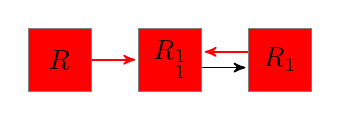
\begin{tikzpicture}[node distance=1.4cm, inner sep=0pt, minimum size=8mm]
        \tikzstyle{seb}=[rectangle, fill=red, draw=gray, text=black]
        \tikzstyle{I1}=[->, draw=red, shorten >=1pt, >=stealth',semithick]
        \tikzstyle{I2}=[->,draw=blue, shorten >=1pt, >=stealth',semithick]
        \tikzstyle{g1}=[->,shorten >=1pt, >=stealth',semithick]
        \tikzstyle{g2}=[->,shorten >=1pt, >=stealth',semithick]
        
        \node[seb] (R0) {$R_{\begin{subarray}{l}\varnothing \\
              \varnothing \end{subarray}}$};
        \node[seb] (R1*) [right of=R0] {$R_{\begin{subarray}{l} 1 \\
              1 \end{subarray}}$};
        \node[seb] (R1) [right of=R1*] {$R_{\begin{subarray}{l} 1 \\
              \varnothing \end{subarray}}$};
        
        % les fleches...
        \draw[I1] (R0) to (R1*);
        \draw[I1] ([yshift=+1mm] R1.west) to ([yshift=+1mm] R1*.east) ; 
        \draw[g1] ([yshift=-1mm] R1*.east) to ([yshift=-1mm] R1.west) ;
        
      \end{tikzpicture}
    \end{column}
    \begin{column}{0.7 \linewidth}
      \begin{itemize}
      \item \alert{$R_{\begin{subarray}{l}H\\ J \end{subarray}}$}; $H$: infectious history (immune repertory)
      \item \alert{$R_{\begin{subarray}{l}H\\ J \end{subarray}}$}; $J$: effective immunity
      \end{itemize}
      
    \end{column}
  \end{columns}
      
  \begin{tiny}
    \begin{align}
      \dot{R}_{\begin{subarray}{l}\varnothing \\
          \varnothing \end{subarray}} &= \mu N -\sum_k \beta_k(t)
      R_{\begin{subarray}{l}\varnothing \\ \varnothing \end{subarray}}
      \frac{I^k}{N} - \mu R_{\begin{subarray}{l}\varnothing \\
          \varnothing \end{subarray}}  \notag \\
      %% 
      \dot{R}_{\begin{subarray}{l}H\\ J \end{subarray}} &= \sum_{k \in
            J} \beta_k \sigma_{Hk} R_{\begin{subarray}{l}H \\ J \setminus
              k \end{subarray}} \frac{I^k}{N} -\sum_{k \in K\setminus J} \beta_k(t)
          \sigma_{Hk} R_{\begin{subarray}{l}H\\ J \end{subarray}}
          \frac{I^k}{N} - \sum_{k \in J} g_k R_{\begin{subarray}{l}H \\
              J \end{subarray}} + \sum_{k \in H \setminus J} g_k
          R_{\begin{subarray}{l}H\\ J\cup k \end{subarray}} -\mu
          R_{\begin{subarray}{l}H\\J \end{subarray}} \notag \\
          %% 
          \dot{I}^k &= \sum_{\begin{subarray}{l}H \subseteq K \\ J
              \subseteq H \setminus k  \end{subarray}} \beta_k
          \sigma_H^k R_{\begin{subarray}{l}H \\ J \end{subarray}}
          \frac{I^k}{N} -\nu I^k -\mu I^k \notag
        \end{align}
      \end{tiny}
      
  \begin{block}{Simplification}
    \begin{itemize}
    \item Focus on the phenotypic level only
    \item Implicit treatment of \alert{within antigenic unit} antigenic drift
    \end{itemize}
  \end{block}
  
\end{frame}


\begin{frame}
  \frametitle{Invasion outcomes (Preliminary study)}
  
  \begin{center}
    \includegraphics<1>[width=0.8 \linewidth]{graph/sens_sout.pdf}
  \end{center}

  \begin{columns}
    \begin{column}{0.5 \linewidth}
      \begin{tiny}
        \begin{itemize}
        \item \textcolor{yellow}{The mutant cannot invade}
        \item \textcolor{green}{Coexistence}
        \item \textcolor{red}{Successfull replacement}
        \item \textcolor{blue}{The mutant only goes extinct after a high
            outbreaks}
        \item Both IAU go extinct
        \end{itemize}
      \end{tiny}
    \end{column}
    \begin{column}{0.5 \linewidth}
      \begin{block}{Conclusion}
        Few parameter areas where \alert{successful IAU replacement occurs}.
      \end{block}
    \end{column}
  \end{columns}

\end{frame}

\begin{frame}
  \frametitle{Confirmation with a realistic context} 
  
  \only<1,2,3,4>{\alert{Metapopulation of 52 major cities in the world}
  \begin{itemize}
  \item<2-> coupling of local dynamics through transportation flows
    (daily air passengers)
  \item<3-> seasonal forcing with phase opposition in North and South
  \item<4-> New IAU are introduced in East Asia every 4 years
  \end{itemize}}



\only<5>{
  \begin{center}
    \begin{footnotesize}
      $R_0=2$; $\sigma_X=0.3$; $\Delta \sigma \in [\alert{0.01}, 0.02, 0.05,
      0.1]$
    \end{footnotesize}
  \end{center}
}
\only<6>{
  \begin{center}
    \begin{footnotesize}
      $R_0=2$; $\sigma_X=0.3$; $\Delta \sigma \in [0.01, \alert{0.02}, 0.05,
      0.1]$
    \end{footnotesize}
  \end{center}
}
\only<7>{
  \begin{center}
    \begin{footnotesize}
      $R_0=2$; $\sigma_X=0.3$; $\Delta \sigma \in [0.01, 0.02, \alert{0.05},
      0.1]$
    \end{footnotesize}
  \end{center}
}
\only<8->{
  \begin{center}
    \begin{footnotesize}
      $R_0=2$; $\sigma_X=0.3$; $\Delta \sigma \in [0.01, 0.02, 0.05,
      \alert{0.1}]$
    \end{footnotesize}
  \end{center}
}

  \begin{center}
    \includegraphics<1>[width=\textwidth]{graph/map00.pdf}
    \includegraphics<2>[width=\textwidth]{graph/map01.pdf}
    \includegraphics<3>[width=\textwidth]{graph/map1.pdf}
    \includegraphics<4>[width=\linewidth]{graph/map2.pdf}
    \includegraphics<5>[width=0.8 \linewidth]{graph/traj_metapop_sout1.pdf}
    \includegraphics<6>[width=0.8 \linewidth]{graph/traj_metapop_sout2.pdf}
    \includegraphics<7>[width=0.8 \linewidth]{graph/traj_metapop_sout3.pdf}
    \includegraphics<8->[width=0.8 \linewidth]{graph/traj_metapop_sout4.pdf}

  \end{center}

%  \begin{block}<3->{}
%    \alert{Contradiction with epochal evolution ?}
%  \end{block}

\end{frame}

\begin{frame}
  \frametitle{Is something missing ?}

  \begin{block}<1->{Data} Current estimates of punctuated immune
    escape ($\Delta \sigma$) are of the order of 15\%
  \end{block}

  \begin{columns}
    \begin{column}{0.5 \linewidth}
      \begin{center}
        \includegraphics<1->[width=0.5\linewidth]{graph/dessin.pdf}
      \end{center}
    \end{column}
    \begin{column}{0.5 \linewidth}
      \begin{center}
        \includegraphics<2->[width=0.5\linewidth]{graph/dessin3.pdf}
      \end{center}
    \end{column}
  \end{columns}

  \begin{alertblock}<2->{Implications of our results}
    \begin{itemize}
    \item<2-> We can reproduce data with $\Delta \sigma <5\%
      \Rightarrow$ antigenic clusters largely overlap.
      \begin{itemize}
      \item<3-> Antigenic evolution is less punctuated that previously
        believed ?
      \item<4-> We miss a process to dampen epidemic intensity following
      immune escape ?
      \end{itemize}
    \end{itemize}
  \end{alertblock}

\end{frame}


\subsection{Additional processes ?}

%\begin{frame}
%  \frametitle{Trade-off between immune escape and intrinsic fitness ($\beta=f(\sigma_{12})$)}
%
%  \only<1->{\begin{tiny} \textcolor{yellow}{Mutant cannot invade};
%    \textcolor{green}{Coexistence}; \textcolor{red}{Successfull
%      replacement}; \textcolor{blue}{Mutant only goes extinct}; Both IAU go extinct \end{tiny}}
%
%  \begin{center}
%    \includegraphics<1>[width=0.8 \linewidth]{graph/trade_off_sout.pdf}
%  \end{center}
%
%\end{frame}

\begin{frame}
  \frametitle{General idea}
  \begin{itemize}
  \item The $SBRI$ model reproduces well antigenic units replacement
    dynamics due to cross-immune boosting process that dampens post
    immune escape epidemics.
  \item This cross-immune boosting process appears unrealistic given
    the existence of original antigenic sin.
  \end{itemize}

  \begin{block}{Question}
    Can we find a related mechanism not in contradiction with original
    antigenic sin ?
  \end{block}

\end{frame}


\begin{frame}
  \frametitle{Temporary strain transcending immunity}

3 different ways to introduce temporary strain transcending immunity
(\alert{$Q$})

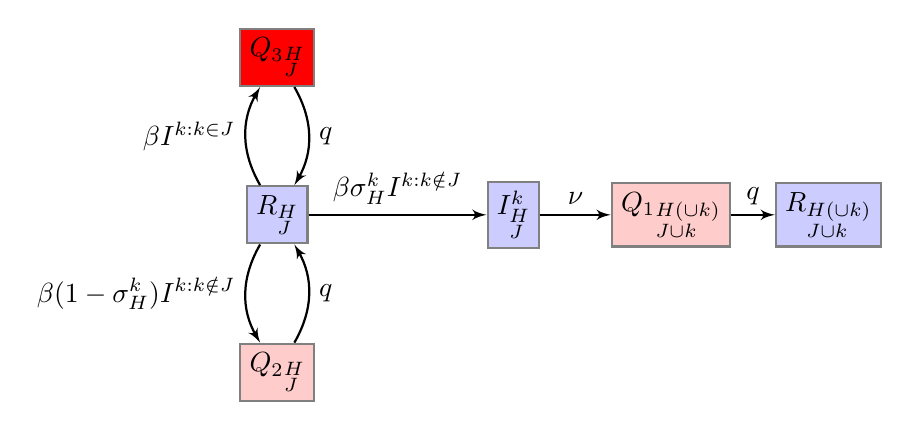
\begin{tikzpicture}[node distance=3cm, auto,>=latex', thick]
  \tikzstyle{sebQ3}=[rectangle, fill=red, draw=gray, text=black]
  \tikzstyle{sebQ}=[rectangle, fill=red!20, draw=gray, text=black]
  \tikzstyle{seb}=[rectangle, fill=blue!20, draw=gray, text=black]
  \node [seb] (X_1_1) {$R_{\begin{subarray}{l}H \\ J\end{subarray}}$};
  \node [seb, right of=X_1_1,node distance=3cm] (I_2_1_1) {$I^{k}_{\begin{subarray}{l}H \\J\end{subarray}}$};
  \node [sebQ, right of=I_2_1_1,node distance=2cm] (Q_12_12) {${Q_1}_{\begin{subarray}{l}H(\cup k) \\J\cup k\end{subarray}}$};
  \node [seb, right of=Q_12_12,node distance=2cm] (X_12_12)
  {$R_{\begin{subarray}{l}H(\cup k) \\J\cup k\end{subarray}}$};

  \draw [->] (X_1_1) --node {$\beta \sigma^k_{H} I^{k:k \notin J}$} (I_2_1_1);
  \draw [->] (I_2_1_1) --node{$\nu$}(Q_12_12);
  \draw [->] (Q_12_12) --node{$q$}(X_12_12);

  \pause
  \node [sebQ, below of=X_1_1,node distance=2cm] (Q2_1_1) {${Q_2}_{\begin{subarray}{l}H \\J\end{subarray}}$};
  \draw [->] (X_1_1) edge[bend right]node[left] {$\beta (1-\sigma^k_{H})I^{k:k \notin J}$} (Q2_1_1);
  \draw [->] (Q2_1_1) edge[bend right]node[right] {$q$} (X_1_1);

  \pause
  \node [sebQ3, above of=X_1_1,node distance=2cm] (Q3_1_1) {${Q_3}_{\begin{subarray}{l}H \\J\end{subarray}}$};  
  \draw [->] (X_1_1) edge[bend left]node[left] {$\beta  I^{k:k \in J}$} (Q3_1_1);
  \draw [->] (Q3_1_1) edge[bend left]node[right] {$q$} (X_1_1);
  
\end{tikzpicture}


\begin{block}{}
  Q2 and Q3 are \alert{immune boosting hypothesis}
\end{block}


\end{frame}



%\begin{frame}
%  \frametitle{Invasion outcome}
%  
%  \begin{tiny} \textcolor{yellow}{Mutant cannot invade};
%    \textcolor{green}{Coexistence}; \textcolor{red}{Successfull
%      replacement}; \textcolor{blue}{Mutant only goes extinct}; Both IAU go extinct \end{tiny}
%
%  \begin{center}
%    \includegraphics<1>[width=0.8 \linewidth]{graph/sens_sout2.pdf}
%    \includegraphics<2>[width=0.8 \linewidth]{graph/sens_sout3.pdf}
%  \end{center}
%
%
%\end{frame}

\begin{frame}
  \frametitle{Importance of immune boosting}

  \begin{columns}
    \begin{column}{0.9 \linewidth}
      \begin{center}
        % \only<1>{
        %   \begin{footnotesize}
        %     $R_0=2$; $\sigma_X=0.3$; $\Delta \sigma \in [0.01, 0.02, 0.05,
        %     0.1]$
        %   \end{footnotesize}
        % } 
        \begin{footnotesize}
          Annual attack rates in Paris; $R_0=5$; $\sigma_X=0.1$; $\Delta \sigma = 0.1$
        \end{footnotesize}
      \end{center}
    \end{column}
    \begin{column}{0.1 \linewidth}
      \begin{flushleft}
        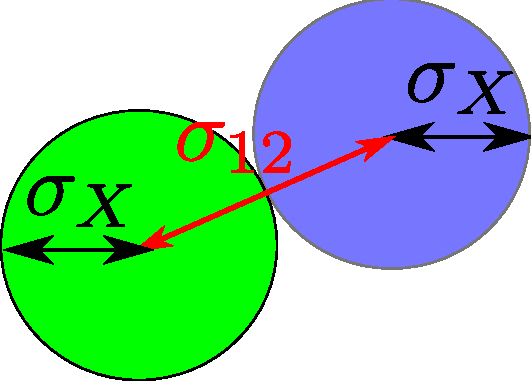
\includegraphics[width=1\linewidth]{graph/dessin4.pdf}
      \end{flushleft}
    \end{column}
  \end{columns}
  
  \begin{center}
    % \includegraphics<1>[width=0.8 \linewidth]{graph/traj_metapop_sout2.pdf}
    \includegraphics<1>[width=0.8 \linewidth]{graph/attack_r05_1.pdf}
    \includegraphics<2>[width=0.8 \linewidth]{graph/attack_r05_2.pdf}
  \end{center}

\end{frame}



\begin{frame}
  \frametitle{Conclusion}
  
  \begin{itemize}
  \item<1-> Core of replacement dynamics is already present in the simple
    $SIRX$ model
  \item<2-> However immune escape results in too high epidemics followed
    by unrealistically long refractory periods with high risks of post
    outbreak extinction
  \item<3-> If we accept influenza antigenic cluster, \alert{``something''
    additional is needed to dampen post-immune escape epidemics}.
    \begin{itemize}
    \item<4-> Heterogeneity at the local level could be a parsimonious explanation
    \item<5-> Immune boosting mechanisms
    \item<6-> Functional constraints such as a trade-off between
      immune escape and intrinsic fitness (\textit{e.g}
      $\beta=f(\Delta \sigma)$)
    \end{itemize}
  \end{itemize}

\end{frame}


\section[UPCA dynamics~~~~~~]{A minimal theory for influenza}

\subsection{Building a minimal model for influenza}


\begin{frame}
  \frametitle{Context}

  \begin{block}{Extrinsic view}
  Antigenic clusters transitions induce epidemic amplitude
  variability, higher peaks reflecting higher antigenic changes    
  \end{block}

  \begin{center}
    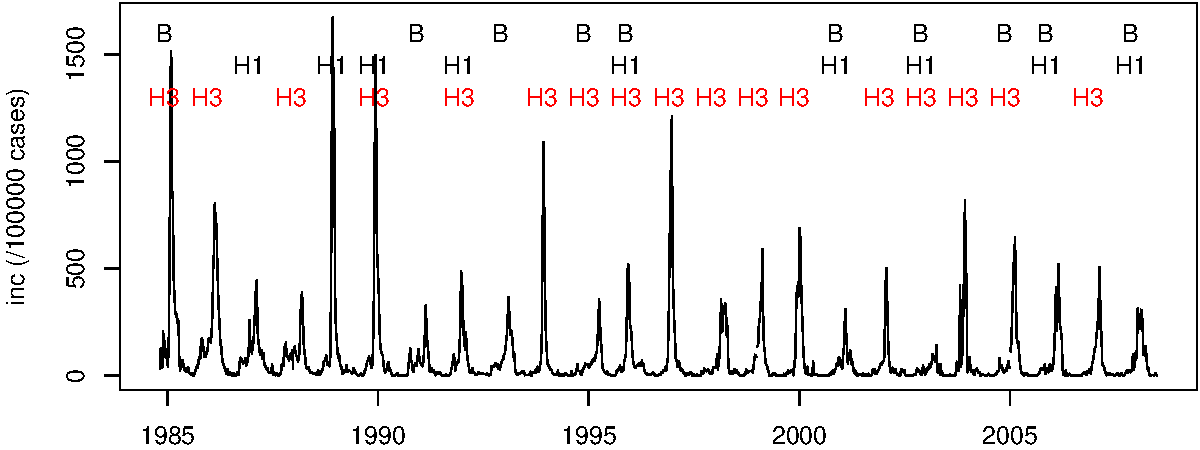
\includegraphics[width=0.7 \linewidth]{graph/data_flu.pdf}
  \end{center}
\pause

  \begin{alertblock}{Intrinsic view}
    Purely gradual antigenic drift and non-linear dynamics alone
    induce Uniform Phase and Chaotic Amplitude (UPCA) dynamics.
  \end{alertblock}
%  \includegraphics<1>[height=0.1 \textwidth]{wolf.png}\\
%  \includegraphics<1>[height=0.1 \textwidth]{koelle.png}
\end{frame}



\begin{frame}
  \frametitle{Building a minimal model: 1- Antigenic drift}
  \begin{center}
    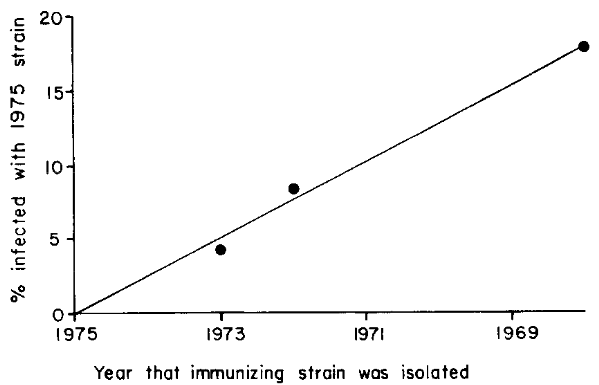
\includegraphics[width=0.4 \linewidth]{graph/pease2.png}
  \end{center}

Classical estimations of \alert{gradual} antigenic drift rate:
  \begin{itemize}
  \item Potter \textit{et. al.} (1977): 19.5 years
  \item Finkenstädt \textit{et. al.} (2005): 13 years (gradual antigenic drift only) or 23.3 years (discrete changes allowed)
  \end{itemize}
\end{frame}



\begin{frame}
  \frametitle{Building a minimal model: 2- A source sink system}
  \begin{center}
    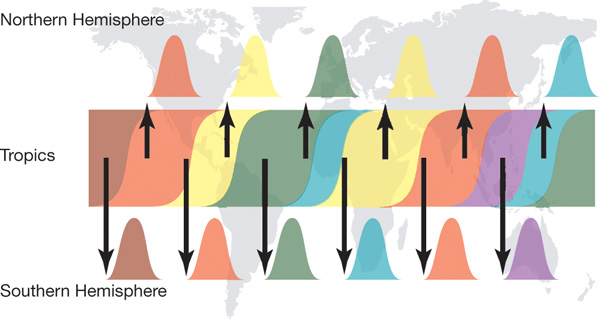
\includegraphics[width=0.8 \linewidth]{graph/rambault.jpg}      

    \begin{tiny} Rambault \textit{et. al.} (2008) \end{tiny}
  \end{center}
\begin{block}{}
  Antigenic changes observed in temperate populations seem to be a
  secondary effect of strong selection within, and largely
  unidirectional flow from, the source population.
\end{block}
\end{frame}


\begin{frame}
  \frametitle{Building a minimal model: 3- Seasonality}
  \begin{center}
    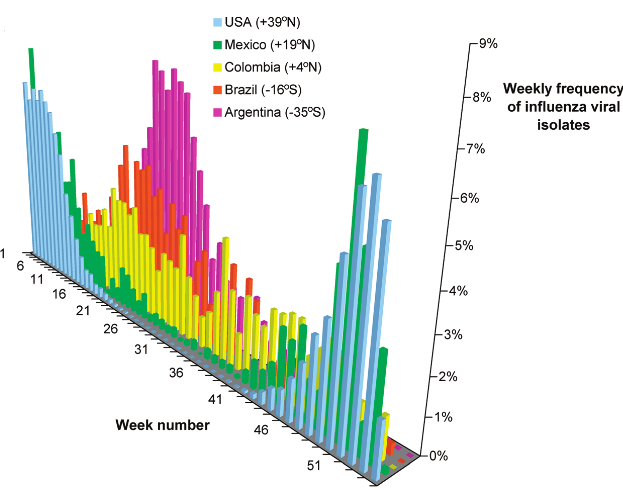
\includegraphics[width=0.8 \linewidth]{graph/viboud.png}
    \begin{tiny} Viboud \textit{et. al.} (2006) \end{tiny}
  \end{center}
\end{frame}


\begin{frame}
  \frametitle{A simple minimal model (intrinsic view)}
  \begin{columns}
    \begin{column}{0.5 \linewidth}
      \begin{center}
        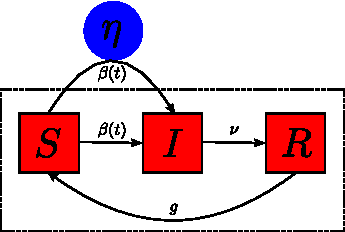
\includegraphics[width=0.7 \linewidth]{graph/sirs.pdf}
      \end{center}
    \end{column}
  \begin{column}{0.5 \linewidth}
  \begin{align*}
    \frac{dS}{dt} &=-\beta_0(1+e \cos(2 \pi t)) \frac{S}{N} (I+\eta) +g R \\
    \frac{dI}{dt} &= \beta_0(1+e \cos(2 \pi t))  \frac{S}{N} (I+\eta) -\nu I \\
    \frac{dR}{dt} &= \nu I -g R
  \end{align*}
  \end{column}
  \end{columns}
\pause

\vspace*{0.5 cm}
Parameters values:
  \begin{itemize}
  \item theoretical parameters (\textit{e.g.} Koelle \textit{et. al.} 2006):\\ $R_0=5$; $1/\nu=8$ days
  \item empirical parameters (\textit{e.g.} Cauchemez \textit{et. al.} 2004): $R_0=2.66$; $1/\nu=2.77$ days
    % \item fitted parameters with \alert{maximum likelihood via iterated
    %     filtering} (Ionides et al. 2006)
    % \item unknown or poorly estimated parameters used as bifurcation
    %   parameters %: $e \in [0,1]$, $1/g \in [2,50]$ years
  \end{itemize}
\end{frame}


\subsection{UPCA dynamics}


%\begin{frame}
%  \frametitle{Locating UPCA dynamics}
%
%We locate UPCA dynamics by:
%\begin{itemize}
%\item a positive first Lyapunov exponent
%\item more than 95 \% of the inter-peak intervals encompassed between
%  0.7 and 1.3 years. Others measures for phase stability do not significantly alter the results.
%\item minimum peaks $> 5\%$ endemic equilibrium value for infectious
%  hosts in the absence of seasonal forcing. This latter criteria
%  ensures that years with small epidemics are nevertheless followed by
%  epidemics (as observed in data)
%\end{itemize}
%
%\end{frame}


\begin{frame}
  \frametitle{Uniform Phase with Chaotic Amplitude dynamics}
    \begin{center}
      \only<1>{Theoretical parameters values}
%      \only<2>{Best fit parameters for IDF data}
      \includegraphics<1>[width=1\textwidth]{graph/pres1upca.pdf}
%      \includegraphics<2>[width=1\textwidth]{graph/pres2upca.pdf}
    \end{center}
\end{frame}



\begin{frame}
  \frametitle{UPCA dynamics occur in wide parameter areas}

  \only<1>{Theoretical and empirical parameters values, unknown parameters used as bifurcation
    parameters}  
%  \only<2>{Support from data: Best fit parameters obtained with \alert{maximum
%    likelihood via iterated filtering}, poorly estimated parameters used as bifurcation
%    parameters}

  \begin{center}
    \includegraphics<1>[width=1\textwidth]{graph/main20.png}
%    \includegraphics<2>[width=1\textwidth]{graph/eta_best_fit2_g11.png}
  \end{center}

\end{frame}


\begin{frame}
  \frametitle{Interacting co-circulating types or subtypes}
  \begin{center}
    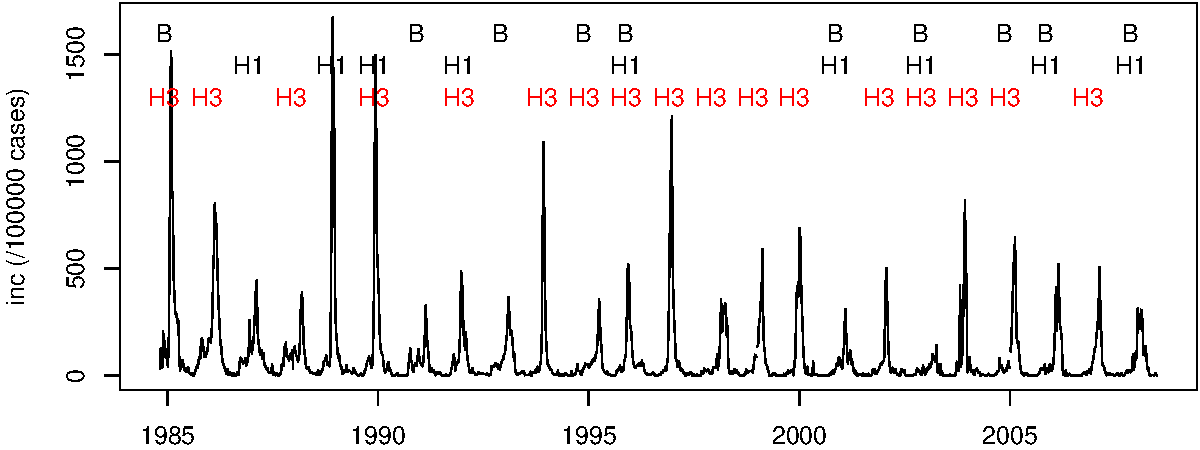
\includegraphics[width=0.8 \linewidth]{graph/data_flu.pdf}    
  \end{center}
  Drifting influenza type and subtype co-circulate. \\ 
  They can interact by: 
  \begin{itemize}
  \item hetero-typic or hetero-subtypic partial cross-immunity
  \item \alert{temporary strain transcending full cross-immunity}
  \end{itemize}
  \pause
  \begin{block}{Question}
    Are UPCA dynamics still present with two cross-reactive
    co-circulating types or subtypes ?
  \end{block}
\end{frame}


\begin{frame}
  \frametitle{UPCA dynamics for influenza co-circulating subtypes}
  
  \begin{center}
    \includegraphics<1>[width=0.8\textwidth]{graph/main2.png}
  \end{center}

  \begin{block}{}
    Subtypes interact only via a temporary period of temporary full cross-immunity    
  \end{block}

\end{frame}



\begin{frame}
  \frametitle{Corroboration from data}
  
  \begin{columns}
    \begin{column}{0.5 \linewidth}
      \begin{center}
        \includegraphics<1>[width=0.9 \textwidth]{graph/all_reconstructed_bernard_theo0.pdf}
        \includegraphics<2>[width=0.9 \textwidth]{graph/all_reconstructed_bernard_theo1.pdf}
        \includegraphics<3>[width=0.9 \textwidth]{graph/all_reconstructed_bernard_theo.pdf}
      \end{center}
    \end{column}
    \begin{column}{0.5 \linewidth}
      \begin{itemize}
      \item<1-> Attractor reconstruction for 2 data sets (Paris area
        and Israel)
      \item<2-> UPCA dynamics with ``refractory period'' for the
        single subtype model \alert{in the absence of antigenic cluster transitions}
      \item<3-> ``Realistic'' dynamics for 2 sub-types model
      \end{itemize}
    \end{column}
  \end{columns}
  
\end{frame}



\subsection{Robustness}


\begin{frame}
  \frametitle{Increasing realism}

  \begin{center}
    %\vspace*{1cm}

    \begin{tikzpicture}[node distance=1.6cm, inner sep=0pt, minimum
      size=10mm, thick]
      % on défini les styles de boites et traits
      \definecolor{monVert}{RGB}{120,212,144}
      % \tikzstyle{erlang} = [draw, fill=sectionColor, rectangle, minimum height=2em, minimum width=3em]
      \tikzstyle{erlang} = [draw, fill=blue!20, rectangle, minimum height=2em, minimum width=3em]
      % \tikzstyle{erlang_2} = [draw, fill=green!20, rectangle, minimum height=2em, minimum width=3em]
      \tikzstyle{erlang_2} = [draw, fill=monVert, rectangle, minimum height=2em, minimum width=3em]
      % \tikzstyle{expo} = [draw, fill=sectionColor, circle,minimum height=2em]
      \tikzstyle{expo} = [draw, fill=blue!20, circle,minimum height=2em]
      % \tikzstyle{expo_2} = [draw, fill=green!20, circle,minimum height=2em]
      \tikzstyle{output} = [coordinate]
      \tikzstyle{expo_2} = [draw, fill=monVert, circle,minimum height=2em]
      \tikzstyle{rouge}=[rectangle, fill=red, draw, text=black]
      \tikzstyle{rougefonce}=[rectangle, fill=red, draw, text=black]
      \tikzstyle{bleu}=[rectangle, fill=blue!20, draw, text=black]
      \tikzstyle{traitrouge}=[->,   draw=red, shorten >=1pt,>=stealth',semithick]
      \tikzstyle{traitbleu}=[->,   draw=blue, shorten >=1pt,>=stealth',semithick]
      \tikzstyle{I2}=[->,draw=blue, shorten >=1pt, >=stealth',semithick]
      \tikzstyle{traitnoir}=[->,shorten >=1pt, >=stealth',semithick]
      \tikzstyle{g2}=[->,shorten >=1pt, >=stealth',semithick]
      % ---------------------------------------------
      
      % We need to set at bounding box first. Otherwise the diagram
      % will change position for each frame.
      %\path[use as bounding box] (-1,0) rectangle (10,-2);
    
      \node<1->[bleu] (sain) {$R_\varnothing$};
      \node<1->[bleu, right of=sain] (expose1) {$E^1_1$};
      \node<1->[bleu, right of=expose1] (expose2) {$E^1_2$};
      \node<1->[bleu, right of=expose2] (infecte1) {$I^1_1$};
      \node<1->[bleu, right of=infecte1] (infecte2) {$I^1_2$};
      \node<1->[rouge, right of=infecte2] (temporary) {$Q^1$};
      \node<1->[bleu, right of=temporary] (immunise) {$R_1$};
      
      \draw<1->[traitrouge] (sain) to (expose1);
      \draw<1->[traitnoir] (expose1) to (expose2);
      \draw<1->[traitnoir] (expose2) to (infecte1);
      \draw<1->[traitnoir] (infecte1) to (infecte2);
      \draw<1->[traitnoir] (infecte2) to (temporary); 
      \draw<1->[traitnoir] (temporary) to (immunise);
     
      \draw<1->[traitbleu](immunise) -- +(0,1) -| node[near start,above] {antigenic drift} (sain);
      
%      \node<1->[rougefonce, below of=infecte1] (infecte_mut){I2};
%      \draw<1->[traitrouge] (sain.south) to (infecte_mut);
%      \draw<1->[traitrouge] (immunise.south) to (infecte_mut);
    
    \end{tikzpicture}
  \end{center}

\begin{small}
  \begin{itemize}
  \item<1-> Erlang distribution for latency ($E$) and infectious period
    ($I$)
  \item<1-> temporary period of full cross protection ($Q$)
  \item<1-> gradual antigenic drift
  \end{itemize}
\end{small}

\begin{alertblock}{co-circulation}
  Coupling of $K$ subtypes, each subtypes modelled with this $SEEIIQRS$ model
\end{alertblock}

\end{frame}

%\begin{frame}
%  \frametitle{Network}
%%  \textcolor{blue}{Metapopulation of 52 major cities in the world}
%  \alert{Metapopulation of 52 major cities in the world}
%  \begin{itemize}
%  \item<2-> coupling of local dynamics through transportation flows
%    (daily air passengers)
%  \item<3-> seasonal forcing with phase opposition in North and South
%  \end{itemize}
%  \begin{center}
%    \includegraphics<1>[width=\textwidth]{graph/map00.pdf}
%    \includegraphics<2>[width=\textwidth]{graph/map01.pdf}
%    \includegraphics<3>[width=\textwidth]{graph/map1.pdf}
%  \end{center}
%\end{frame}

\begin{frame}
  \frametitle{Realistic migrations  and Heterogeneous contacts}
  \alert{Three age classes} within 52 world major cities coupled through transportation flows
    (daily air passengers)
  \begin{itemize}
    \item realistic contact matrix and demographic data
  \end{itemize}
    \begin{center}
      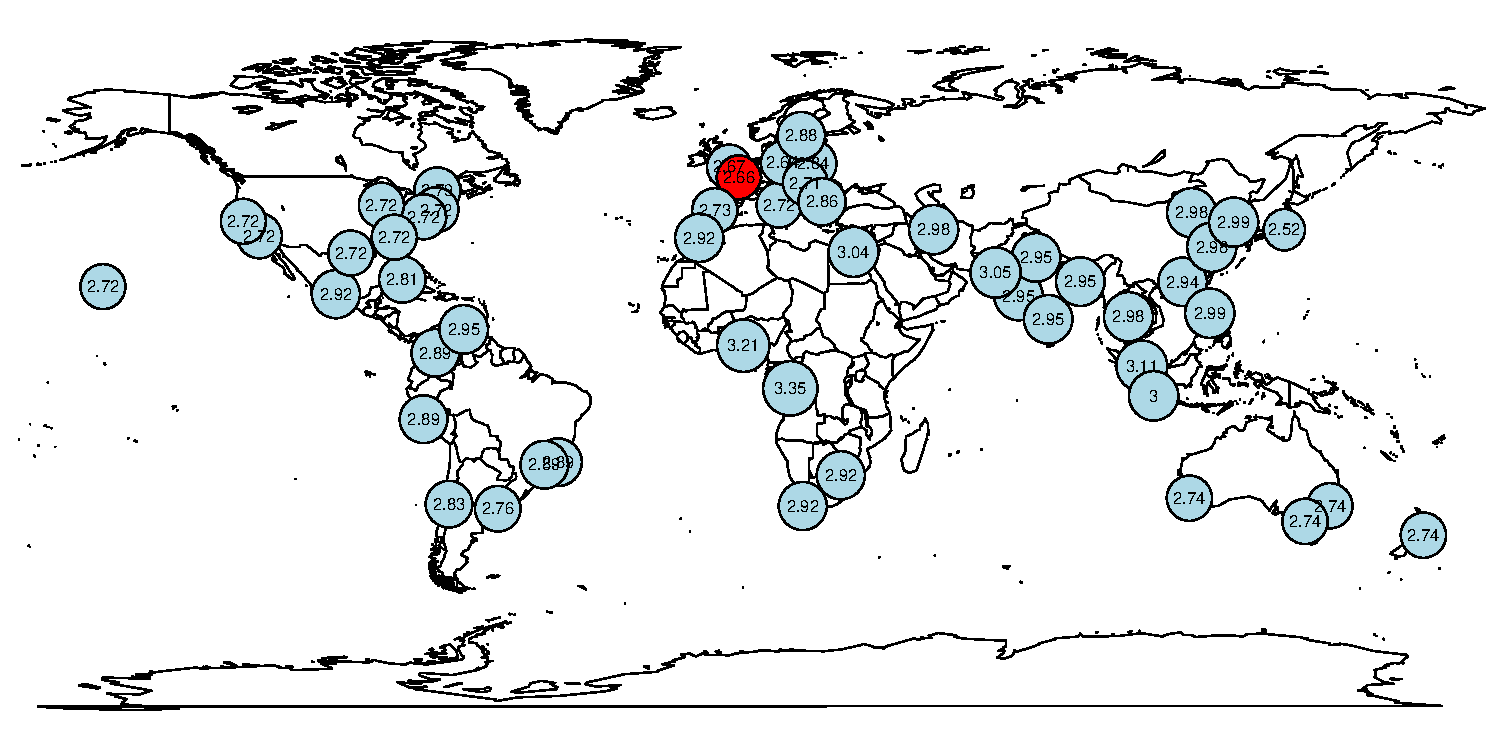
\includegraphics[width=\textwidth]{graph/r0_mex.pdf}
    \end{center}
\end{frame}
%Local $R_0$ of A/H1N1


\begin{frame}
  \frametitle{Technical aspects}
  \alert{Stochastic} model in continuous time, Markovian
  transitions, simulations performed using an Euler-multinomial approximation

\begin{tiny}
\begin{align}
%  \label{eq:app2:full}
%%R
\dot{R}_{\begin{subarray}{l}J\\ a_i, c_l \end{subarray}} &=  q Q_{\begin{subarray}{l}J  \\ a_i,
    c_l \end{subarray}} - \sum_{k \notin J} \sigma_{a_i}^k \beta_k(t)
\frac{R_{\begin{subarray}{l}J\\ a_i, c_l \end{subarray}}}{p_{a_i} N_{c_l}} \sum_j M_{ij}
I^k_{a_j,c_l} -\sum_{k
  \in J} g_k R_{\begin{subarray}{l}J\\ a_i, c_l \end{subarray}} + \sum_{k
  \notin J} g_k R_{\begin{subarray}{l}J \cup k \\ a_i, c_l \end{subarray}} \notag \\
%%
%%E
\dot{E_1}^k_{\begin{subarray}{l}J \setminus k\\ a_i,
    c_l \end{subarray}} &=\sigma_{a_i}^k \beta_k(t)
\frac{R_{\begin{subarray}{l}J \setminus k\\ a_i, c_l \end{subarray}}}{p_{a_i} N_{c_l}} \sum_j M_{ij}
I^k_{a_j,c_l} -2 \gamma {E_1}^k_{\begin{subarray}{l}J
    \setminus k\\ a_i, c_l \end{subarray}} -\sum_{m\neq l}
\frac{p_{a_i} \tau_{c_lc_m}}{N_{c_l}} {E_1}^k_{\begin{subarray}{l}J \setminus k\\ a_i,
    c_l \end{subarray}} -\sum_{m
  \in J \setminus k} g_m {E_1}^k_{\begin{subarray}{l}J \setminus k\\ a_i, c_l \end{subarray}} + \sum_{m
  \notin J \setminus k} g_m {E_1}^k_{\begin{subarray}{l} (J \setminus k) \cup m \\ a_i, c_l \end{subarray}} 
\notag \\
%%
%%E'
\dot{E_2}^k_{\begin{subarray}{l}J \setminus k\\ a_i, c_l \end{subarray}}
&=2 \gamma {E_1}^k_{\begin{subarray}{l}J \setminus k\\ a_i,
    c_l \end{subarray}} -2 \gamma {E_2}^k_{\begin{subarray}{l}J \setminus k\\ a_i, c_l \end{subarray}}
+\sum_{m\neq l} \frac{p_{a_i} \tau_{c_mc_l}}{N_{c_l}} {E_1}^k_{\begin{subarray}{l}J \setminus k\\ a_i,
    c_m \end{subarray}} -\sum_{m\neq l} \frac{p_{a_i}  \tau_{c_lc_m}}{N_{c_l}} {E_2}^k_{\begin{subarray}{l}J \setminus k\\ a_i,
    c_l \end{subarray}} -\sum_{m
  \in J \setminus k} g_m {E_2}^k_{\begin{subarray}{l}J \setminus k\\ a_i, c_l \end{subarray}} + \sum_{m
  \notin J \setminus k} g_m {E_2}^k_{\begin{subarray}{l} (J \setminus k) \cup m \\ a_i, c_l \end{subarray}}  \notag \\
%%
%%I
\dot{I_1}^k_{\begin{subarray}{l}J \setminus k\\ a_i, c_l \end{subarray}} &=2 \gamma {E_2}^k_{\begin{subarray}{l}J \setminus k\\ a_i, c_l \end{subarray}}
-2 \nu {I_1}^k_{\begin{subarray}{l}J \setminus k\\ a_i,
    c_l \end{subarray}} + \sum_{m\neq l} \frac{p_{a_i} \tau_{c_mc_l}}{N_{c_l}} {E_2}^k_{\begin{subarray}{l}J \setminus k\\ a_i,
    c_m \end{subarray}}  -\sum_{m
  \in J \setminus k} g_m {I_1}^k_{\begin{subarray}{l}J \setminus k\\ a_i, c_l \end{subarray}} + \sum_{m
  \notin J \setminus k} g_m {I_1}^k_{\begin{subarray}{l} (J \setminus k) \cup m \\ a_i, c_l \end{subarray}}  \notag \\
%%
%%I'
\dot{I_2}^k_{\begin{subarray}{l}J \setminus k\\ a_i,
    c_l \end{subarray}} &=2 \nu {I_1}^k_{\begin{subarray}{l}J:k
    \notin J\\ a_i, c_l \end{subarray}} -2 \nu {I_2}^k_{\begin{subarray}{l}J \setminus k\\ a_i, c_l \end{subarray}} -\sum_{m
  \in J \setminus k} g_m {I_2}^k_{\begin{subarray}{l}J \setminus k\\ a_i, c_l \end{subarray}} + \sum_{m
  \notin J \setminus k} g_m {I_2}^k_{\begin{subarray}{l} (J \setminus k) \cup m \\ a_i, c_l \end{subarray}} 
\notag \\
%%
%%Q
\dot{Q}^k_{\begin{subarray}{l}J \\ a_i, c_l \end{subarray}}
&= \sum_{k \in J} 2 \nu {I_2}^k_{\begin{subarray}{l}J \setminus k\\
    a_i,
    c_l \end{subarray}} - q Q_{\begin{subarray}{l}J \\
    a_i, c_l \end{subarray}} -\sum_{k \in J} g_k
Q_{\begin{subarray}{l}J\\ a_i, c_l \end{subarray}} + \sum_{k \notin J}
g_k Q_{\begin{subarray}{l}J \cup k \\ a_i, c_l \end{subarray}} \notag
\end{align}
\end{tiny}

\end{frame}




\begin{frame}
  \frametitle{UPCA dynamics persist}
  
  Typical realisation of the stochastic metapopulation model with
  \alert{realistic migration scenario}, age structure and
  non-exponential duration of infection for the city of Paris.

\begin{itemize}
\item<1-> Total weekly incidence (for both subtypes \textit{e.g} H3N2 and H1N1)
\item<2-> Weekly incidence per subtype \alert{H3N2} and \textcolor{blue}{H1N1}
\end{itemize}

  \begin{center}
    \includegraphics<1>[width=1\textwidth]{graph/metapopupca0.pdf}
    \includegraphics<2->[width=1\textwidth]{graph/metapopupca1.pdf}
  \end{center}
  
\end{frame}



\begin{frame}
  \frametitle{Conclusion}
    \begin{itemize}
    \item<1-> Non-linear dynamics alone can explain the observed
      pattern of influenza recurrence.
    \item<2-> UPCA dynamics appears to be robust to various
      perturbations.
    \item<3-> Higher epidemic peaks cannot therefore be taken as a
      signature of punctually large antigenic changes as they can
      result from intrinsic mechanisms.
    \item<4-> If the intrinsic view is correct, fundamental
      unpredictability of future epidemic sizes in addition to
      evolutionary contingency.
    \end{itemize}

    \begin{alertblock}<5->{Proposition}
      UPCA dynamics as a minimal model for influenza.
    \end{alertblock}

\end{frame}


\section{Discussion}

\subsection{Gradual or punctuated antigenic evolution}

\begin{frame}
  \frametitle{Main determinant of influenza phylodynamics}

  \begin{block}{Signatures from data}
    \begin{itemize}
    \item \alert{\sout{Regular recurrent epidemics with variable amplitudes}}
    \item Slender phylogenetic tree with limited diversity at any time
    \item Hemagglutination assay, antigenic map
    \item Subtypes replacement/coexistence during pandemics
    \end{itemize}
  \end{block}
  
\pause

  \begin{block}{Theory}
    \begin{enumerate}
    \item \alert{Punctuated immune escape must be accompanied with immune
      boosting and/or a form of heterogeneity}
    \item Q class without immune boosting must be accompanied of a
      form of heterogeneity (Tria \textit{et al.} 2005)
    \end{enumerate}
  \end{block}

\pause

  \begin{alertblock}{}
    2 main hypothesis explaining limited strains diversity need
    \textcolor{blue}{additional source of heterogeneity} and/or
    \alert{immune boosting}.
  \end{alertblock}

\end{frame}

\begin{frame}
  \frametitle{Perspectives}

  \begin{block}{Population level}
    \begin{itemize}
    \item Statistical inference with \alert{Maximum likelihood via Iterated
        Filtering} using the SIRX framework.
    \item 2 statistical tests of the nature of influenza antigenic
      evolution
    \item Work in progress with Katia Koelle, Anton Camacho and
      Bernard Cazelles
    \end{itemize}
%    Ideally feed with data from tropics
  \end{block}

\pause

\begin{alertblock}{Intra-host level}
  Clarification of immunological processes in particular the complex
  interplay of humoral and cellular immune response in the context of
  original antigenic sin and sequential effects.
\end{alertblock}

\end{frame}



\subsection{Implications for pandemics}



\begin{frame}
  \frametitle{Implication for pandemics}
  
  \begin{block}{Temporary full /Partial cross immunity}
    \begin{itemize}
    \item Due to possible importance of immune boosting we should not
      assume that population is fully susceptible even in case of
      pandemics.
    \item The $SIRX$ model suggests important hetero-subtypic cross
      protection. \alert{Implication for $R_0$ inference}
    \end{itemize}
  \end{block}

\pause

  \begin{alertblock}{Importance of number of infections}
    \begin{itemize}
    \item Study of pandemics in a fully naive population (\textit{e.g}
      Tristan da Cunha) reveals importance of multiple infections
      before acquiring long term immunity.
      \begin{tikzpicture}[node distance=2cm, auto,>=latex', thick]<1>
        \tikzstyle{seb}=[->,draw=red, shorten >=1pt, >=stealth',semithick]
        \node [naif] (S) {$S$};
        \node [expo, right of=S] (I) {$I$};
        \node [expo, right of=I] (Q) {$Q$};
        \node [expo, right of=Q] (R) {$R$};
        % \node [mut, below of=R] (I2) {$I_2$};
        % \node [mut, below of=X] (I2) {$I_2$};
        
        % Once the nodes are placed, connecting them is easy. 
        \draw [->] (S) -- node {$\beta$} (I);
        \draw [->] (I) -- node{$\nu$}(Q);
        \draw [seb] (Q) -- node{\alert{$\alpha q$}}(R);
        \draw [seb](Q) -- +(0,1) -| node[near start,below] {\alert{$(1-\alpha) q$}} (S);
      \end{tikzpicture}
    \end{itemize} 
  \end{alertblock}
  

\end{frame}


\begin{frame}
  \frametitle{Application of our minimal model for predicting nao H1N1
    pandemic subtype invasion outcome}
  
  \begin{center}
    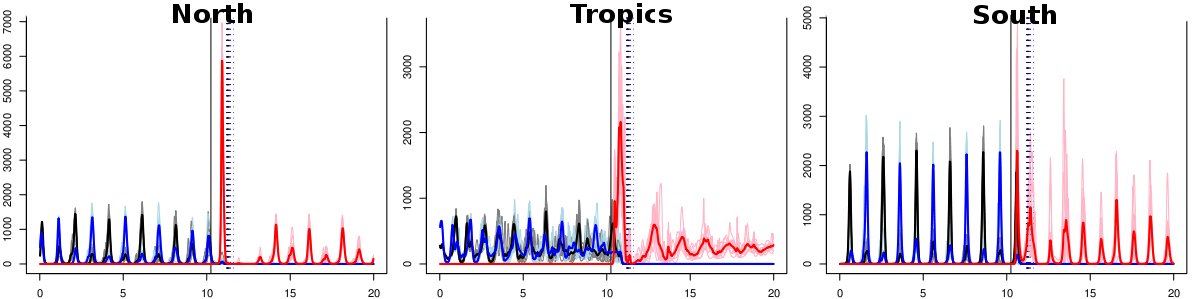
\includegraphics[width=0.9\textwidth]{graph/traj_replace.png}
  \end{center}

  \begin{footnotesize}
    Seasonal \textcolor{blue}{H1N1}, H3N2 subtypes co-circulate and on
    April (time=10), the \alert{new animal origin H1N1} pandemic
    subtype is introduced in Mexico.
  \end{footnotesize}

  \pause

  \begin{footnotesize}
  \begin{block}{Preliminary results}
    \begin{itemize}
    \item Strong tendency for replacements for wide parameters area
      ($R_0$(s) and antigenic drift rates)
    \item \alert{But..} Importance of initial conditions (old individuals and adults
      can be partially protected to the pandemic subtype independently
      of the $Q$ classes)
    \end{itemize}
  \end{block}
  \end{footnotesize}

\end{frame}





%%%%%%%%%%%%%
%%%%%%%%%%%%%
%%%%%%%%%%%%%



\begin{frame}
  \frametitle{Thanks}
%\vspace*{2 cm}
  \begin{center} 
    \includegraphics<1>[width=1 \linewidth]{graph/thanks.pdf}
%    Thank you for your attention !
 \end{center}
%\vspace*{3 cm}
%Work supported by Region Ile de France\\
%\includegraphics<1>[width=0.3 \linewidth]{graph/idf.jpg}
\end{frame}



%%%%%%%%%%%%%%%%%%%%%%%%%%%%%%%%%%%%%%%%%%%%%%%%%%%%%%%%%%%%%
%%%%%%%%%%%%%%%%%%%%%%%%%%%%%%%%%%%%%%%%%%%%%%%%%%%%%%%%%%%%%
%%%%%%%%%%%%%%%%%%%%%%%%%%%%%%%%%%%%%%%%%%%%%%%%%%%%%%%%%%%%%
%%%%%%%%%%%%%%%%%%%%%%%%%%%%%%%%%%%%%%%%%%%%%%%%%%%%%%%%%%%%%
%%%%%%%%%%%%%%%%%%%%%%%%%%%%%%%%%%%%%%%%%%%%%%%%%%%%%%%%%%%%%
%%%%%%%%%%%%%%%%%%%%%FINI%%%%%%%%%%%%%%%%%%%%%%%%%%%%%%%%%%%%
%%%%%%%%%%%%%%%%%%%%%%%%%%%%%%%%%%%%%%%%%%%%%%%%%%%%%%%%%%%%%
%%%%%%%%%%%%%%%%%%%%%%%%%%%%%%%%%%%%%%%%%%%%%%%%%%%%%%%%%%%%%
%%%%%%%%%%%%%%%%%%%%%%%%%%%%%%%%%%%%%%%%%%%%%%%%%%%%%%%%%%%%%
%%%%%%%%%%%%%%%%%%%%%%%%%%%%%%%%%%%%%%%%%%%%%%%%%%%%%%%%%%%%%
%%%%%%%%%%%%%%%%%%%%%%%%%%%%%%%%%%%%%%%%%%%%%%%%%%%%%%%%%%%%%
%%%%%%%%%%%%%%%%%%%%%%%%%%%%%%%%%%%%%%%%%%%%%%%%%%%%%%%%%%%%%





\appendix



\begin{frame}
  \frametitle{Lange \& Ferguson 2009 model}
  
\only<1->{Immune escape (\alert{antigenic variability}) at the intra-host level influence infection duration.}

  \begin{columns}
    \begin{column}{0.5 \linewidth}<2->
      \begin{itemize}
      \item<2-> cross-immunity
      \item<3-> infectiousness threshold $P_T$:  $\beta(t)=q(1-\exp(-\frac{P}{P_T}))$
      \item<4-> key role of trade-off between reproductive rate and
        antigenic mutability
      \end{itemize}
    \end{column}
    \begin{column}{0.5 \linewidth}<3->
      \includegraphics<3>[width=1 \linewidth]{graph/lange_hiv.jpg}    
      \includegraphics<4->[width=1 \linewidth]{graph/lange.jpg}    
    \end{column}
  \end{columns}

\end{frame}



\begin{frame}
  \frametitle{Drawbacks of history based model: lack of memory}

  \begin{columns}
    \begin{column}{0.3 \linewidth}
      
  \begin{tikzpicture}[node distance=1.7cm, inner sep=0pt, minimum size=8mm]
    \tikzstyle{seb}=[rectangle, fill=red, draw=gray, text=black]
    \tikzstyle{I1}=[->, draw=red, shorten >=1pt, >=stealth',semithick]
    \tikzstyle{I2}=[->,draw=blue, shorten >=1pt, >=stealth',semithick]
    \tikzstyle{g1}=[->,shorten >=1pt, >=stealth',semithick]
    \tikzstyle{g2}=[->,shorten >=1pt, >=stealth',semithick]

    \node[seb] (R0) {$R_\varnothing$}; 
    \node[seb] (R1) [above of=R0] {$R_1$};
    \node[seb] (R2) [below of=R0] {$R_2$};
    \node[seb] (R12) [right of=R0] {$R_{12}$};

    \draw[I1] (R0) to node[auto] {\begin{tiny}$\beta R_\varnothing I^1$\end{tiny}} (R1);
    \draw[I2] (R0) to node[auto,swap] {\begin{tiny}$\beta R_\varnothing I^2$\end{tiny}} (R2);
    \draw[I2] ([yshift=+4mm] R1.east) to node[auto] {\begin{tiny}$\sigma_{12} \beta R_1 I^2$\end{tiny}} ([yshift=+4mm] R12.west); 
    \draw[I1] ([yshift=-4mm] R2.east) to node[auto,swap] {\begin{tiny}$\sigma_{12} \beta R_2 I^1$\end{tiny}} ([yshift=-4mm] R12.west);

    \pause
    \draw[g1] ([xshift=+2mm] R1.south) to node[auto] {\begin{tiny}$\gamma_1 \gamma_2$\end{tiny}} ([xshift=+2mm] R0.north); 
    \draw[g2] ([xshift=+2mm] R2.north) to node[auto,swap] {\begin{tiny}$\gamma_2 \gamma_1$\end{tiny}} ([xshift=+2mm] R0.south) ;
    \draw[g1] (R12.west) to (R2.east) ;
    \draw[g2] (R12.west) to (R1.east) ;
  \end{tikzpicture}  

    \end{column}
    \begin{column}{0.7 \linewidth}
      \begin{itemize}
      \item If IAU $i$ evolves we loose the fact that $R_i$ hosts (now
        $R_\varnothing$) are partially protected to the second IAU.
      \item This assumption would be relevant for waning immunity but in our case
        contradicts the fact that influenza specific immune response appears
        to be long-lived.
      \item The memory of partial protection is important to
        take into account as the IAU can be considered separated by a fixed
        antigenic distance that remains constant despite within IAU evolution.
      \end{itemize}
    \end{column}
  \end{columns}

\end{frame}



\begin{frame}
  \frametitle{Immune boosting and Status based models}
  \begin{columns}
    \begin{column}{0.5 \linewidth}
      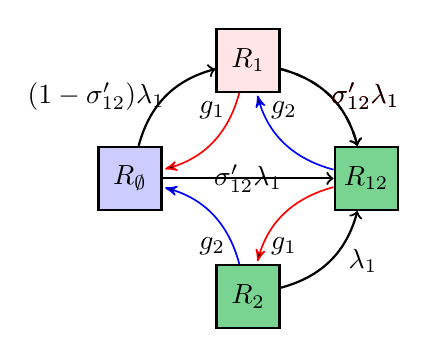
\begin{tikzpicture}[node distance=1.5cm, thick, inner sep=0pt, minimum size=8mm]
        \definecolor{monVert}{RGB}{120,212,144}
        \tikzstyle{class_X} = [draw, fill=blue!20, rectangle]
        \tikzstyle{class_X_2} = [draw, fill=monVert, rectangle]
        \tikzstyle{class_X_3} = [draw, fill=red!10, rectangle]
        \tikzstyle{I2}=[->,draw=red, shorten >=1pt, >=stealth',semithick]    
        \tikzstyle{I1}=[->,draw=blue, shorten >=1pt, >=stealth',semithick]
        \tikzstyle{output} = [coordinate]
        
        \node<1-> [class_X] (R0) {$R_{\emptyset}$};	
        \node<1-> [class_X_2, right of=R0,node distance=3cm] (R12) {$R_{12}$};
        \draw<1-> [->] (R0) --node[name=R0R12] {$\sigma'_{12}\lambda_1$}(R12);
        \node<1-> [class_X_3, above of=R0R12] (R1) {$R_1$};
        \node<1-> [class_X_2, below of=R0R12] (R2) {$R_2$};
        \draw<1-> [->] (R0) edge[bend left]node[left]{$(1-\sigma'_{12})\lambda_1$}(R1);
        \draw<2-> [I2] (R1) edge[bend left]node[above]{$g_{1}$}(R0);
        \draw<2-> [I2] (R12) edge[bend right]node[below]{$g_{1}$}(R2);
        \draw<2-> [->] (R2) edge[bend right]node[right]{$\lambda_1$}(R12);

        \draw<4-> [I1] (R2) edge[bend right]node[below]{$g_{2}$}(R0);
        \draw<4-> [I1] (R12) edge[bend left]node[above]{$g_{2}$}(R1);
        
        \draw<1> [->] (R1) edge[bend left]node[right]{$\textcolor{red}{\sigma'_{12}\lambda_1}$}(R12);
        \draw<2-> [->] (R1) edge[bend left, dashed]node[right]{$\sigma'_{12}\lambda_1$}(R12);
      \end{tikzpicture}
      
    \end{column}
    \begin{column}{0.5 \linewidth}
      \includegraphics<3>[width= 0.7 \linewidth]{graph/threshold_koelle.pdf}      
      \includegraphics<4>[width= 0.7 \linewidth]{graph/threshold_koelle2.pdf}      
    \end{column}
  \end{columns}


  \begin{footnotesize}
    \begin{itemize}
    \item<3,4-> Strong Invasion threshold depending on the ability of the
      mutant cluster to drift before its appearance in a given area
      \begin{itemize}
      \item<3-> Clusters give rise to each others: $g_2=0$ before 2
        introduction $\Rightarrow$ invasion threshold
      \item<4-> Mutant drift in another place before its introduction:
        $g_2=g_1$ before 2 introduction $\Rightarrow$ no invasion
        threshold and ``loss'' of meaning for immune escape (SBRS model)
      \end{itemize}
    \end{itemize}
  \end{footnotesize}
\end{frame}



\begin{frame}
  \frametitle{Endemic equilibrium of the  $SIRX$ model}

  \begin{center}
    \includegraphics<1->[width=0.9 \linewidth]{graph/eq_end_sout.pdf}
  \end{center}

  \begin{block}{}
    Strong dynamical impact of the \alert{reinfection threshold
      ($\sigma_X=1/R_0$)}.
  \end{block}

\end{frame}


\begin{frame}
  \frametitle{Invasion threshold of the $SIRX$ model}
  
  \begin{center}
    \includegraphics<1>[width=0.9 \linewidth]{graph/threshold_sout.pdf}
  \end{center}


  \begin{block}{Sufficient condition to allow invasion of a mutant IAU}
    \alert{$\sigma_{12}>\sigma_X$} $\Rightarrow$ Infection by a given IAU confers a better
    protection against strains belonging to the same IAU than against
    strains of another IAU.
  \end{block}

\end{frame}


\begin{frame}
  \frametitle{Invasion outcome $SIRX$, $SIRXQ1$, $SIRXQ12$ models}
  
  \begin{tiny} \textcolor{yellow}{Mutant cannot invade};
    \textcolor{green}{Coexistence}; \textcolor{red}{Successfull
      replacement}; \textcolor{blue}{Mutant only goes extinct}; Both IAU go extinct \end{tiny}

  \begin{center}
    \includegraphics<1>[width=0.8 \linewidth]{graph/sens_sout2.pdf}
    \includegraphics<2>[width=0.8 \linewidth]{graph/sens_sout3.pdf}
  \end{center}


\end{frame}


\end{document}